\documentclass[twoside]{book}

% Packages required by doxygen
\usepackage{fixltx2e}
\usepackage{calc}
\usepackage{doxygen}
\usepackage[export]{adjustbox} % also loads graphicx
\usepackage{graphicx}
\usepackage[utf8]{inputenc}
\usepackage{makeidx}
\usepackage{multicol}
\usepackage{multirow}
\PassOptionsToPackage{warn}{textcomp}
\usepackage{textcomp}
\usepackage[nointegrals]{wasysym}
\usepackage[table]{xcolor}

% Font selection
\usepackage[T1]{fontenc}
\usepackage[scaled=.90]{helvet}
\usepackage{courier}
\usepackage{amssymb}
\usepackage{sectsty}
\renewcommand{\familydefault}{\sfdefault}
\allsectionsfont{%
  \fontseries{bc}\selectfont%
  \color{darkgray}%
}
\renewcommand{\DoxyLabelFont}{%
  \fontseries{bc}\selectfont%
  \color{darkgray}%
}
\newcommand{\+}{\discretionary{\mbox{\scriptsize$\hookleftarrow$}}{}{}}

% Page & text layout
\usepackage{geometry}
\geometry{%
  a4paper,%
  top=2.5cm,%
  bottom=2.5cm,%
  left=2.5cm,%
  right=2.5cm%
}
\tolerance=750
\hfuzz=15pt
\hbadness=750
\setlength{\emergencystretch}{15pt}
\setlength{\parindent}{0cm}
\setlength{\parskip}{3ex plus 2ex minus 2ex}
\makeatletter
\renewcommand{\paragraph}{%
  \@startsection{paragraph}{4}{0ex}{-1.0ex}{1.0ex}{%
    \normalfont\normalsize\bfseries\SS@parafont%
  }%
}
\renewcommand{\subparagraph}{%
  \@startsection{subparagraph}{5}{0ex}{-1.0ex}{1.0ex}{%
    \normalfont\normalsize\bfseries\SS@subparafont%
  }%
}
\makeatother

% Headers & footers
\usepackage{fancyhdr}
\pagestyle{fancyplain}
\fancyhead[LE]{\fancyplain{}{\bfseries\thepage}}
\fancyhead[CE]{\fancyplain{}{}}
\fancyhead[RE]{\fancyplain{}{\bfseries\leftmark}}
\fancyhead[LO]{\fancyplain{}{\bfseries\rightmark}}
\fancyhead[CO]{\fancyplain{}{}}
\fancyhead[RO]{\fancyplain{}{\bfseries\thepage}}
\fancyfoot[LE]{\fancyplain{}{}}
\fancyfoot[CE]{\fancyplain{}{}}
\fancyfoot[RE]{\fancyplain{}{\bfseries\scriptsize Generated by Doxygen }}
\fancyfoot[LO]{\fancyplain{}{\bfseries\scriptsize Generated by Doxygen }}
\fancyfoot[CO]{\fancyplain{}{}}
\fancyfoot[RO]{\fancyplain{}{}}
\renewcommand{\footrulewidth}{0.4pt}
\renewcommand{\chaptermark}[1]{%
  \markboth{#1}{}%
}
\renewcommand{\sectionmark}[1]{%
  \markright{\thesection\ #1}%
}

% Indices & bibliography
\usepackage{natbib}
\usepackage[titles]{tocloft}
\setcounter{tocdepth}{3}
\setcounter{secnumdepth}{5}
\makeindex

% Hyperlinks (required, but should be loaded last)
\usepackage{ifpdf}
\ifpdf
  \usepackage[pdftex,pagebackref=true]{hyperref}
\else
  \usepackage[ps2pdf,pagebackref=true]{hyperref}
\fi
\hypersetup{%
  colorlinks=true,%
  linkcolor=blue,%
  citecolor=blue,%
  unicode%
}

% Custom commands
\newcommand{\clearemptydoublepage}{%
  \newpage{\pagestyle{empty}\cleardoublepage}%
}

\usepackage{caption}
\captionsetup{labelsep=space,justification=centering,font={bf},singlelinecheck=off,skip=4pt,position=top}

%===== C O N T E N T S =====

\begin{document}

% Titlepage & ToC
\hypersetup{pageanchor=false,
             bookmarksnumbered=true,
             pdfencoding=unicode
            }
\pagenumbering{alph}
\begin{titlepage}
\vspace*{7cm}
\begin{center}%
{\Large 3D Assignment One }\\
\vspace*{1cm}
{\large Generated by Doxygen 1.8.13}\\
\end{center}
\end{titlepage}
\clearemptydoublepage
\pagenumbering{roman}
\tableofcontents
\clearemptydoublepage
\pagenumbering{arabic}
\hypersetup{pageanchor=true}

%--- Begin generated contents ---
\chapter{Hierarchical Index}
\section{Class Hierarchy}
This inheritance list is sorted roughly, but not completely, alphabetically\+:\begin{DoxyCompactList}
\item Frame\+Listener\begin{DoxyCompactList}
\item \contentsline{section}{Base\+Application}{\pageref{class_base_application}}{}
\begin{DoxyCompactList}
\item \contentsline{section}{Basic\+Tutorial\+\_\+00}{\pageref{class_basic_tutorial__00}}{}
\end{DoxyCompactList}
\end{DoxyCompactList}
\item Key\+Listener\begin{DoxyCompactList}
\item \contentsline{section}{Base\+Application}{\pageref{class_base_application}}{}
\end{DoxyCompactList}
\item Mouse\+Listener\begin{DoxyCompactList}
\item \contentsline{section}{Base\+Application}{\pageref{class_base_application}}{}
\end{DoxyCompactList}
\item Sdk\+Tray\+Listener\begin{DoxyCompactList}
\item \contentsline{section}{Base\+Application}{\pageref{class_base_application}}{}
\end{DoxyCompactList}
\item Window\+Event\+Listener\begin{DoxyCompactList}
\item \contentsline{section}{Base\+Application}{\pageref{class_base_application}}{}
\end{DoxyCompactList}
\end{DoxyCompactList}

\chapter{Class Index}
\section{Class List}
Here are the classes, structs, unions and interfaces with brief descriptions\+:\begin{DoxyCompactList}
\item\contentsline{section}{\hyperlink{class_base_application}{Base\+Application} }{\pageref{class_base_application}}{}
\item\contentsline{section}{\hyperlink{class_basic_tutorial__00}{Basic\+Tutorial\+\_\+00} \\*3D Game Programming ~\newline
My Name\+: Li-\/\+Che Chien ~\newline
My ID\+: 0316235 ~\newline
My Email\+: \href{mailto:richard@hotmail.com}{\tt richard@hotmail.\+com} }{\pageref{class_basic_tutorial__00}}{}
\end{DoxyCompactList}

\chapter{File Index}
\section{File List}
Here is a list of all files with brief descriptions\+:\begin{DoxyCompactList}
\item\contentsline{section}{\hyperlink{_base_application_8cpp}{Base\+Application.\+cpp} }{\pageref{_base_application_8cpp}}{}
\item\contentsline{section}{\hyperlink{_base_application_8h}{Base\+Application.\+h} }{\pageref{_base_application_8h}}{}
\item\contentsline{section}{\hyperlink{_tutorial_application_8cpp}{Tutorial\+Application.\+cpp} }{\pageref{_tutorial_application_8cpp}}{}
\item\contentsline{section}{\hyperlink{_tutorial_application_8h}{Tutorial\+Application.\+h} }{\pageref{_tutorial_application_8h}}{}
\end{DoxyCompactList}

\chapter{Class Documentation}
\hypertarget{class_base_application}{}\section{Base\+Application Class Reference}
\label{class_base_application}\index{Base\+Application@{Base\+Application}}


{\ttfamily \#include $<$Base\+Application.\+h$>$}

Inheritance diagram for Base\+Application\+:\begin{figure}[H]
\begin{center}
\leavevmode
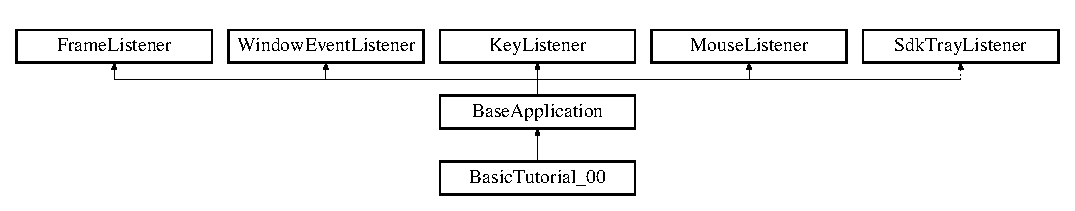
\includegraphics[height=2.382979cm]{class_base_application}
\end{center}
\end{figure}
\subsection*{Public Member Functions}
\begin{DoxyCompactItemize}
\item 
\hyperlink{class_base_application_a7c897f08816cc064568ae1ec71026719}{Base\+Application} (void)
\item 
virtual \hyperlink{class_base_application_a48e1966307d5ef8f6cbf8b6e980ad652}{$\sim$\+Base\+Application} (void)
\item 
virtual void \hyperlink{class_base_application_a8a14a65a29118dd75173aa68678a05e1}{go} (void)
\end{DoxyCompactItemize}
\subsection*{Protected Member Functions}
\begin{DoxyCompactItemize}
\item 
virtual bool \hyperlink{class_base_application_a5853d0e148cb85b0297a6885e1d33a89}{setup} ()
\item 
virtual bool \hyperlink{class_base_application_a62ed46f90e9f82cc810997647a2c587e}{configure} (void)
\item 
virtual void \hyperlink{class_base_application_ad5bc9655041e1849a4c13f444a3712bd}{choose\+Scene\+Manager} (void)
\item 
virtual void \hyperlink{class_base_application_afa9d51527763cf9aee9cd4e1b1039d55}{create\+Camera} (void)
\item 
virtual void \hyperlink{class_base_application_aff6fd9ff1ff0978cc68f19dd65be4778}{create\+Frame\+Listener} (void)
\item 
virtual void \hyperlink{class_base_application_aa97beeb4059b17d0ec22eae33286ec2d}{create\+Scene} (void)=0
\item 
virtual void \hyperlink{class_base_application_a365146059b25391fe400f5fdb94f011e}{destroy\+Scene} (void)
\item 
virtual void \hyperlink{class_base_application_a1f8f6730cae6ec769d8730b1af48486e}{create\+Viewports} (void)
\item 
virtual void \hyperlink{class_base_application_ae27301702f1e5de64619a39b1929f1f9}{setup\+Resources} (void)
\item 
virtual void \hyperlink{class_base_application_a9b77972f0f747a61e1f8ceba2ad47641}{create\+Resource\+Listener} (void)
\item 
virtual void \hyperlink{class_base_application_aaeb764e637dd87601a81a80156659d88}{load\+Resources} (void)
\item 
virtual bool \hyperlink{class_base_application_a03912a0f38b38fede7f08a2571e8fc56}{frame\+Rendering\+Queued} (const Ogre\+::\+Frame\+Event \&evt)
\item 
virtual bool \hyperlink{class_base_application_acfa977f04e435f18018ece805c1277ec}{key\+Pressed} (const O\+I\+S\+::\+Key\+Event \&arg)
\item 
virtual bool \hyperlink{class_base_application_aba5c7c9dea7a0efc58b89310bae547e5}{key\+Released} (const O\+I\+S\+::\+Key\+Event \&arg)
\item 
virtual bool \hyperlink{class_base_application_a126e59cb246b061e51eb6ce06a2ee8f4}{mouse\+Moved} (const O\+I\+S\+::\+Mouse\+Event \&arg)
\item 
virtual bool \hyperlink{class_base_application_a9255dfc1eabefd11c474ec45a6622504}{mouse\+Pressed} (const O\+I\+S\+::\+Mouse\+Event \&arg, O\+I\+S\+::\+Mouse\+Button\+ID id)
\item 
virtual bool \hyperlink{class_base_application_aa102c5859c14c0690c749994a446b53d}{mouse\+Released} (const O\+I\+S\+::\+Mouse\+Event \&arg, O\+I\+S\+::\+Mouse\+Button\+ID id)
\item 
virtual void \hyperlink{class_base_application_afacf8a797588592ef0abbad593f10cfa}{window\+Resized} (Ogre\+::\+Render\+Window $\ast$rw)
\item 
virtual void \hyperlink{class_base_application_ae0e37ac54a31ff6e51d58c7654ad1b90}{window\+Closed} (Ogre\+::\+Render\+Window $\ast$rw)
\end{DoxyCompactItemize}
\subsection*{Protected Attributes}
\begin{DoxyCompactItemize}
\item 
Ogre\+::\+Root $\ast$ \hyperlink{class_base_application_add84ba707dc6c57e6283f214b1274110}{m\+Root}
\item 
Ogre\+::\+Camera $\ast$ \hyperlink{class_base_application_a3829c6b12afe911e97e6b4524b33a38b}{m\+Camera}
\item 
Ogre\+::\+Scene\+Manager $\ast$ \hyperlink{class_base_application_a8a7684f4f9a57ed3089048ad1a913b2d}{m\+Scene\+Mgr}
\item 
Ogre\+::\+Render\+Window $\ast$ \hyperlink{class_base_application_ac5d8e9c81e036897bc82f81eff8c570f}{m\+Window}
\item 
Ogre\+::\+String \hyperlink{class_base_application_a765e0df01c141a16df3178ab4f17afe6}{m\+Resources\+Cfg}
\item 
Ogre\+::\+String \hyperlink{class_base_application_a04f2fe47fa164fd78d986dc0df70b7fb}{m\+Plugins\+Cfg}
\item 
Ogre\+Bites\+::\+Sdk\+Tray\+Manager $\ast$ \hyperlink{class_base_application_a7faa397f4f4861ee8c361a01e90b4416}{m\+Tray\+Mgr}
\item 
Ogre\+Bites\+::\+Sdk\+Camera\+Man $\ast$ \hyperlink{class_base_application_a9ae38dea6316058549151fff66a91fcd}{m\+Camera\+Man}
\item 
Ogre\+Bites\+::\+Params\+Panel $\ast$ \hyperlink{class_base_application_a6a11054ca61efdf558e0ff1b2de43a12}{m\+Details\+Panel}
\item 
bool \hyperlink{class_base_application_ac7e861799862cb645f1d78b170aef80d}{m\+Cursor\+Was\+Visible}
\item 
bool \hyperlink{class_base_application_a755f26d3a9915aaf830750d877e39d86}{m\+Shut\+Down}
\item 
O\+I\+S\+::\+Input\+Manager $\ast$ \hyperlink{class_base_application_abc9503c8462e225b5d0d55c952d9e4a9}{m\+Input\+Manager}
\item 
O\+I\+S\+::\+Mouse $\ast$ \hyperlink{class_base_application_add9b97fbe64da2814d3af113bac58c43}{m\+Mouse}
\item 
O\+I\+S\+::\+Keyboard $\ast$ \hyperlink{class_base_application_a9d6e19cf50c47379fbaae55bff28079c}{m\+Keyboard}
\end{DoxyCompactItemize}


\subsection{Constructor \& Destructor Documentation}
\mbox{\Hypertarget{class_base_application_a7c897f08816cc064568ae1ec71026719}\label{class_base_application_a7c897f08816cc064568ae1ec71026719}} 
\index{Base\+Application@{Base\+Application}!Base\+Application@{Base\+Application}}
\index{Base\+Application@{Base\+Application}!Base\+Application@{Base\+Application}}
\subsubsection{\texorpdfstring{Base\+Application()}{BaseApplication()}}
{\footnotesize\ttfamily Base\+Application\+::\+Base\+Application (\begin{DoxyParamCaption}\item[{void}]{ }\end{DoxyParamCaption})}


\begin{DoxyCode}
21     : \hyperlink{class_base_application_add84ba707dc6c57e6283f214b1274110}{mRoot}(0),
22     \hyperlink{class_base_application_a3829c6b12afe911e97e6b4524b33a38b}{mCamera}(0),
23     \hyperlink{class_base_application_a8a7684f4f9a57ed3089048ad1a913b2d}{mSceneMgr}(0),
24     \hyperlink{class_base_application_ac5d8e9c81e036897bc82f81eff8c570f}{mWindow}(0),
25     \hyperlink{class_base_application_a765e0df01c141a16df3178ab4f17afe6}{mResourcesCfg}(Ogre::StringUtil::BLANK),
26     \hyperlink{class_base_application_a04f2fe47fa164fd78d986dc0df70b7fb}{mPluginsCfg}(Ogre::StringUtil::BLANK),
27     \hyperlink{class_base_application_a7faa397f4f4861ee8c361a01e90b4416}{mTrayMgr}(0),
28     \hyperlink{class_base_application_a9ae38dea6316058549151fff66a91fcd}{mCameraMan}(0),
29     \hyperlink{class_base_application_a6a11054ca61efdf558e0ff1b2de43a12}{mDetailsPanel}(0),
30     \hyperlink{class_base_application_ac7e861799862cb645f1d78b170aef80d}{mCursorWasVisible}(\textcolor{keyword}{true}),
31     \hyperlink{class_base_application_a755f26d3a9915aaf830750d877e39d86}{mShutDown}(\textcolor{keyword}{false}),
32     \hyperlink{class_base_application_abc9503c8462e225b5d0d55c952d9e4a9}{mInputManager}(0),
33     \hyperlink{class_base_application_add9b97fbe64da2814d3af113bac58c43}{mMouse}(0),
34     \hyperlink{class_base_application_a9d6e19cf50c47379fbaae55bff28079c}{mKeyboard}(0)
35 \{
36 \}
\end{DoxyCode}
\mbox{\Hypertarget{class_base_application_a48e1966307d5ef8f6cbf8b6e980ad652}\label{class_base_application_a48e1966307d5ef8f6cbf8b6e980ad652}} 
\index{Base\+Application@{Base\+Application}!````~Base\+Application@{$\sim$\+Base\+Application}}
\index{````~Base\+Application@{$\sim$\+Base\+Application}!Base\+Application@{Base\+Application}}
\subsubsection{\texorpdfstring{$\sim$\+Base\+Application()}{~BaseApplication()}}
{\footnotesize\ttfamily Base\+Application\+::$\sim$\+Base\+Application (\begin{DoxyParamCaption}\item[{void}]{ }\end{DoxyParamCaption})\hspace{0.3cm}{\ttfamily [virtual]}}



References m\+Camera\+Man, m\+Root, m\+Tray\+Mgr, m\+Window, and window\+Closed().


\begin{DoxyCode}
40 \{
41     \textcolor{keywordflow}{if} (\hyperlink{class_base_application_a7faa397f4f4861ee8c361a01e90b4416}{mTrayMgr}) \textcolor{keyword}{delete} \hyperlink{class_base_application_a7faa397f4f4861ee8c361a01e90b4416}{mTrayMgr};
42     \textcolor{keywordflow}{if} (\hyperlink{class_base_application_a9ae38dea6316058549151fff66a91fcd}{mCameraMan}) \textcolor{keyword}{delete} \hyperlink{class_base_application_a9ae38dea6316058549151fff66a91fcd}{mCameraMan};
43 
44     \textcolor{comment}{//Remove ourself as a Window listener}
45     Ogre::WindowEventUtilities::removeWindowEventListener(\hyperlink{class_base_application_ac5d8e9c81e036897bc82f81eff8c570f}{mWindow}, \textcolor{keyword}{this});
46     \hyperlink{class_base_application_ae0e37ac54a31ff6e51d58c7654ad1b90}{windowClosed}(\hyperlink{class_base_application_ac5d8e9c81e036897bc82f81eff8c570f}{mWindow});
47     \textcolor{keyword}{delete} \hyperlink{class_base_application_add84ba707dc6c57e6283f214b1274110}{mRoot};
48 \}
\end{DoxyCode}


\subsection{Member Function Documentation}
\mbox{\Hypertarget{class_base_application_ad5bc9655041e1849a4c13f444a3712bd}\label{class_base_application_ad5bc9655041e1849a4c13f444a3712bd}} 
\index{Base\+Application@{Base\+Application}!choose\+Scene\+Manager@{choose\+Scene\+Manager}}
\index{choose\+Scene\+Manager@{choose\+Scene\+Manager}!Base\+Application@{Base\+Application}}
\subsubsection{\texorpdfstring{choose\+Scene\+Manager()}{chooseSceneManager()}}
{\footnotesize\ttfamily void Base\+Application\+::choose\+Scene\+Manager (\begin{DoxyParamCaption}\item[{void}]{ }\end{DoxyParamCaption})\hspace{0.3cm}{\ttfamily [protected]}, {\ttfamily [virtual]}}



Reimplemented in \hyperlink{class_basic_tutorial__00_aba97a29d983586d2dc8e108d3bccf721}{Basic\+Tutorial\+\_\+00}.



References m\+Root, and m\+Scene\+Mgr.



Referenced by setup().


\begin{DoxyCode}
71 \{
72     \textcolor{comment}{// Get the SceneManager, in this case a generic one}
73     \hyperlink{class_base_application_a8a7684f4f9a57ed3089048ad1a913b2d}{mSceneMgr} = \hyperlink{class_base_application_add84ba707dc6c57e6283f214b1274110}{mRoot}->createSceneManager(Ogre::ST\_GENERIC);
74 \}
\end{DoxyCode}
\mbox{\Hypertarget{class_base_application_a62ed46f90e9f82cc810997647a2c587e}\label{class_base_application_a62ed46f90e9f82cc810997647a2c587e}} 
\index{Base\+Application@{Base\+Application}!configure@{configure}}
\index{configure@{configure}!Base\+Application@{Base\+Application}}
\subsubsection{\texorpdfstring{configure()}{configure()}}
{\footnotesize\ttfamily bool Base\+Application\+::configure (\begin{DoxyParamCaption}\item[{void}]{ }\end{DoxyParamCaption})\hspace{0.3cm}{\ttfamily [protected]}, {\ttfamily [virtual]}}



References m\+Root, and m\+Window.



Referenced by setup().


\begin{DoxyCode}
52 \{
53     \textcolor{comment}{// Show the configuration dialog and initialise the system}
54     \textcolor{comment}{// You can skip this and use root.restoreConfig() to load configuration}
55     \textcolor{comment}{// settings if you were sure there are valid ones saved in ogre.cfg}
56     \textcolor{keywordflow}{if}(\hyperlink{class_base_application_add84ba707dc6c57e6283f214b1274110}{mRoot}->showConfigDialog())
57     \{
58         \textcolor{comment}{// If returned true, user clicked OK so initialise}
59         \textcolor{comment}{// Here we choose to let the system create a default rendering window by passing 'true'}
60         \hyperlink{class_base_application_ac5d8e9c81e036897bc82f81eff8c570f}{mWindow} = \hyperlink{class_base_application_add84ba707dc6c57e6283f214b1274110}{mRoot}->initialise(\textcolor{keyword}{true}, \textcolor{stringliteral}{"NCTU. 3D Game Programming. Student Name: ²�߭�.
       ID:0316235"});
61 
62         \textcolor{keywordflow}{return} \textcolor{keyword}{true};
63     \}
64     \textcolor{keywordflow}{else}
65     \{
66         \textcolor{keywordflow}{return} \textcolor{keyword}{false};
67     \}
68 \}
\end{DoxyCode}
\mbox{\Hypertarget{class_base_application_afa9d51527763cf9aee9cd4e1b1039d55}\label{class_base_application_afa9d51527763cf9aee9cd4e1b1039d55}} 
\index{Base\+Application@{Base\+Application}!create\+Camera@{create\+Camera}}
\index{create\+Camera@{create\+Camera}!Base\+Application@{Base\+Application}}
\subsubsection{\texorpdfstring{create\+Camera()}{createCamera()}}
{\footnotesize\ttfamily void Base\+Application\+::create\+Camera (\begin{DoxyParamCaption}\item[{void}]{ }\end{DoxyParamCaption})\hspace{0.3cm}{\ttfamily [protected]}, {\ttfamily [virtual]}}



Reimplemented in \hyperlink{class_basic_tutorial__00_a1bf709417d654dffc2ea10987412b912}{Basic\+Tutorial\+\_\+00}.



References m\+Camera, m\+Camera\+Man, and m\+Scene\+Mgr.



Referenced by setup().


\begin{DoxyCode}
77 \{
78     \textcolor{comment}{// Create the camera}
79     \hyperlink{class_base_application_a3829c6b12afe911e97e6b4524b33a38b}{mCamera} = \hyperlink{class_base_application_a8a7684f4f9a57ed3089048ad1a913b2d}{mSceneMgr}->createCamera(\textcolor{stringliteral}{"PlayerCam"});
80 
81     \textcolor{comment}{/*}
82 \textcolor{comment}{    // Position it at 500 in Z direction}
83 \textcolor{comment}{    mCamera->setPosition(Ogre::Vector3(0,0,80));}
84 \textcolor{comment}{    // Look back along -Z}
85 \textcolor{comment}{    mCamera->lookAt(Ogre::Vector3(0,0,-300));}
86 \textcolor{comment}{    */}
87 
88     
89     \hyperlink{class_base_application_a3829c6b12afe911e97e6b4524b33a38b}{mCamera}->setPosition(Ogre::Vector3(0,80,1000));
90     \hyperlink{class_base_application_a3829c6b12afe911e97e6b4524b33a38b}{mCamera}->lookAt(Ogre::Vector3(0,0,0));
91 
92     \hyperlink{class_base_application_a3829c6b12afe911e97e6b4524b33a38b}{mCamera}->setNearClipDistance(5);
93 
94     \hyperlink{class_base_application_a9ae38dea6316058549151fff66a91fcd}{mCameraMan} = \textcolor{keyword}{new} OgreBites::SdkCameraMan(\hyperlink{class_base_application_a3829c6b12afe911e97e6b4524b33a38b}{mCamera});   \textcolor{comment}{// create a default camera
       controller}
95 \}
\end{DoxyCode}
\mbox{\Hypertarget{class_base_application_aff6fd9ff1ff0978cc68f19dd65be4778}\label{class_base_application_aff6fd9ff1ff0978cc68f19dd65be4778}} 
\index{Base\+Application@{Base\+Application}!create\+Frame\+Listener@{create\+Frame\+Listener}}
\index{create\+Frame\+Listener@{create\+Frame\+Listener}!Base\+Application@{Base\+Application}}
\subsubsection{\texorpdfstring{create\+Frame\+Listener()}{createFrameListener()}}
{\footnotesize\ttfamily void Base\+Application\+::create\+Frame\+Listener (\begin{DoxyParamCaption}\item[{void}]{ }\end{DoxyParamCaption})\hspace{0.3cm}{\ttfamily [protected]}, {\ttfamily [virtual]}}



References m\+Details\+Panel, m\+Input\+Manager, m\+Keyboard, m\+Mouse, m\+Root, m\+Tray\+Mgr, m\+Window, and window\+Resized().



Referenced by setup().


\begin{DoxyCode}
98 \{
99     Ogre::LogManager::getSingletonPtr()->logMessage(\textcolor{stringliteral}{"*** Initializing OIS ***"});
100     OIS::ParamList pl;
101     \textcolor{keywordtype}{size\_t} windowHnd = 0;
102     std::ostringstream windowHndStr;
103 
104     \hyperlink{class_base_application_ac5d8e9c81e036897bc82f81eff8c570f}{mWindow}->getCustomAttribute(\textcolor{stringliteral}{"WINDOW"}, &windowHnd);
105     windowHndStr << windowHnd;
106     pl.insert(std::make\_pair(std::string(\textcolor{stringliteral}{"WINDOW"}), windowHndStr.str()));
107 
108     \hyperlink{class_base_application_abc9503c8462e225b5d0d55c952d9e4a9}{mInputManager} = OIS::InputManager::createInputSystem( pl );
109 
110     \hyperlink{class_base_application_a9d6e19cf50c47379fbaae55bff28079c}{mKeyboard} = \textcolor{keyword}{static\_cast<}OIS::Keyboard*\textcolor{keyword}{>}(\hyperlink{class_base_application_abc9503c8462e225b5d0d55c952d9e4a9}{mInputManager}->createInputObject( 
      OIS::OISKeyboard, \textcolor{keyword}{true} ));
111     \hyperlink{class_base_application_add9b97fbe64da2814d3af113bac58c43}{mMouse} = \textcolor{keyword}{static\_cast<}OIS::Mouse*\textcolor{keyword}{>}(\hyperlink{class_base_application_abc9503c8462e225b5d0d55c952d9e4a9}{mInputManager}->createInputObject( OIS::OISMouse, \textcolor{keyword}{
      true} ));
112 
113     \hyperlink{class_base_application_add9b97fbe64da2814d3af113bac58c43}{mMouse}->setEventCallback(\textcolor{keyword}{this});
114     \hyperlink{class_base_application_a9d6e19cf50c47379fbaae55bff28079c}{mKeyboard}->setEventCallback(\textcolor{keyword}{this});
115 
116     \textcolor{comment}{//Set initial mouse clipping size}
117     \hyperlink{class_base_application_afacf8a797588592ef0abbad593f10cfa}{windowResized}(\hyperlink{class_base_application_ac5d8e9c81e036897bc82f81eff8c570f}{mWindow});
118 
119     \textcolor{comment}{//Register as a Window listener}
120     Ogre::WindowEventUtilities::addWindowEventListener(\hyperlink{class_base_application_ac5d8e9c81e036897bc82f81eff8c570f}{mWindow}, \textcolor{keyword}{this});
121 
122     \hyperlink{class_base_application_a7faa397f4f4861ee8c361a01e90b4416}{mTrayMgr} = \textcolor{keyword}{new} OgreBites::SdkTrayManager(\textcolor{stringliteral}{"InterfaceName"}, \hyperlink{class_base_application_ac5d8e9c81e036897bc82f81eff8c570f}{mWindow}, 
      \hyperlink{class_base_application_add9b97fbe64da2814d3af113bac58c43}{mMouse}, \textcolor{keyword}{this});
123     \hyperlink{class_base_application_a7faa397f4f4861ee8c361a01e90b4416}{mTrayMgr}->showFrameStats(OgreBites::TL\_BOTTOMLEFT);
124     \hyperlink{class_base_application_a7faa397f4f4861ee8c361a01e90b4416}{mTrayMgr}->showLogo(OgreBites::TL\_BOTTOMRIGHT);
125     \textcolor{comment}{//mTrayMgr->hideCursor();}
126     \hyperlink{class_base_application_a7faa397f4f4861ee8c361a01e90b4416}{mTrayMgr}->showCursor();
127 
128     \textcolor{comment}{// create a params panel for displaying sample details}
129     Ogre::StringVector items;
130     items.push\_back(\textcolor{stringliteral}{"cam.pX"});
131     items.push\_back(\textcolor{stringliteral}{"cam.pY"});
132     items.push\_back(\textcolor{stringliteral}{"cam.pZ"});
133     items.push\_back(\textcolor{stringliteral}{""});
134     items.push\_back(\textcolor{stringliteral}{"cam.oW"});
135     items.push\_back(\textcolor{stringliteral}{"cam.oX"});
136     items.push\_back(\textcolor{stringliteral}{"cam.oY"});
137     items.push\_back(\textcolor{stringliteral}{"cam.oZ"});
138     items.push\_back(\textcolor{stringliteral}{""});
139     items.push\_back(\textcolor{stringliteral}{"Filtering"});
140     items.push\_back(\textcolor{stringliteral}{"Poly Mode"});
141 
142     \hyperlink{class_base_application_a6a11054ca61efdf558e0ff1b2de43a12}{mDetailsPanel} = \hyperlink{class_base_application_a7faa397f4f4861ee8c361a01e90b4416}{mTrayMgr}->createParamsPanel(OgreBites::TL\_NONE, \textcolor{stringliteral}{"DetailsPanel"}, 20
      0, items);
143     \hyperlink{class_base_application_a6a11054ca61efdf558e0ff1b2de43a12}{mDetailsPanel}->setParamValue(9, \textcolor{stringliteral}{"Bilinear"});
144     \hyperlink{class_base_application_a6a11054ca61efdf558e0ff1b2de43a12}{mDetailsPanel}->setParamValue(10, \textcolor{stringliteral}{"Solid"});
145     \hyperlink{class_base_application_a6a11054ca61efdf558e0ff1b2de43a12}{mDetailsPanel}->hide();
146 
147     \hyperlink{class_base_application_add84ba707dc6c57e6283f214b1274110}{mRoot}->addFrameListener(\textcolor{keyword}{this});
148 \}
\end{DoxyCode}
\mbox{\Hypertarget{class_base_application_a9b77972f0f747a61e1f8ceba2ad47641}\label{class_base_application_a9b77972f0f747a61e1f8ceba2ad47641}} 
\index{Base\+Application@{Base\+Application}!create\+Resource\+Listener@{create\+Resource\+Listener}}
\index{create\+Resource\+Listener@{create\+Resource\+Listener}!Base\+Application@{Base\+Application}}
\subsubsection{\texorpdfstring{create\+Resource\+Listener()}{createResourceListener()}}
{\footnotesize\ttfamily void Base\+Application\+::create\+Resource\+Listener (\begin{DoxyParamCaption}\item[{void}]{ }\end{DoxyParamCaption})\hspace{0.3cm}{\ttfamily [protected]}, {\ttfamily [virtual]}}



Referenced by setup().


\begin{DoxyCode}
191 \{
192 
193 \}
\end{DoxyCode}
\mbox{\Hypertarget{class_base_application_aa97beeb4059b17d0ec22eae33286ec2d}\label{class_base_application_aa97beeb4059b17d0ec22eae33286ec2d}} 
\index{Base\+Application@{Base\+Application}!create\+Scene@{create\+Scene}}
\index{create\+Scene@{create\+Scene}!Base\+Application@{Base\+Application}}
\subsubsection{\texorpdfstring{create\+Scene()}{createScene()}}
{\footnotesize\ttfamily virtual void Base\+Application\+::create\+Scene (\begin{DoxyParamCaption}\item[{void}]{ }\end{DoxyParamCaption})\hspace{0.3cm}{\ttfamily [protected]}, {\ttfamily [pure virtual]}}



Implemented in \hyperlink{class_basic_tutorial__00_a15a3d4673724ec99077ce992f996a550}{Basic\+Tutorial\+\_\+00}.



Referenced by setup().

\mbox{\Hypertarget{class_base_application_a1f8f6730cae6ec769d8730b1af48486e}\label{class_base_application_a1f8f6730cae6ec769d8730b1af48486e}} 
\index{Base\+Application@{Base\+Application}!create\+Viewports@{create\+Viewports}}
\index{create\+Viewports@{create\+Viewports}!Base\+Application@{Base\+Application}}
\subsubsection{\texorpdfstring{create\+Viewports()}{createViewports()}}
{\footnotesize\ttfamily void Base\+Application\+::create\+Viewports (\begin{DoxyParamCaption}\item[{void}]{ }\end{DoxyParamCaption})\hspace{0.3cm}{\ttfamily [protected]}, {\ttfamily [virtual]}}



Reimplemented in \hyperlink{class_basic_tutorial__00_adc2454d9f8226e0958ecf702f355846e}{Basic\+Tutorial\+\_\+00}.



References m\+Camera, and m\+Window.



Referenced by setup().


\begin{DoxyCode}
155 \{
156     \textcolor{comment}{// Create one viewport, entire window}
157     Ogre::Viewport* vp = \hyperlink{class_base_application_ac5d8e9c81e036897bc82f81eff8c570f}{mWindow}->addViewport(\hyperlink{class_base_application_a3829c6b12afe911e97e6b4524b33a38b}{mCamera});
158     vp->setBackgroundColour(Ogre::ColourValue(0,0,0));
159 
160     \textcolor{comment}{// Alter the camera aspect ratio to match the viewport}
161     \hyperlink{class_base_application_a3829c6b12afe911e97e6b4524b33a38b}{mCamera}->setAspectRatio(
162         Ogre::Real(vp->getActualWidth()) / Ogre::Real(vp->getActualHeight()));
163 \}
\end{DoxyCode}
\mbox{\Hypertarget{class_base_application_a365146059b25391fe400f5fdb94f011e}\label{class_base_application_a365146059b25391fe400f5fdb94f011e}} 
\index{Base\+Application@{Base\+Application}!destroy\+Scene@{destroy\+Scene}}
\index{destroy\+Scene@{destroy\+Scene}!Base\+Application@{Base\+Application}}
\subsubsection{\texorpdfstring{destroy\+Scene()}{destroyScene()}}
{\footnotesize\ttfamily void Base\+Application\+::destroy\+Scene (\begin{DoxyParamCaption}\item[{void}]{ }\end{DoxyParamCaption})\hspace{0.3cm}{\ttfamily [protected]}, {\ttfamily [virtual]}}



Referenced by go().


\begin{DoxyCode}
151 \{
152 \}
\end{DoxyCode}
\mbox{\Hypertarget{class_base_application_a03912a0f38b38fede7f08a2571e8fc56}\label{class_base_application_a03912a0f38b38fede7f08a2571e8fc56}} 
\index{Base\+Application@{Base\+Application}!frame\+Rendering\+Queued@{frame\+Rendering\+Queued}}
\index{frame\+Rendering\+Queued@{frame\+Rendering\+Queued}!Base\+Application@{Base\+Application}}
\subsubsection{\texorpdfstring{frame\+Rendering\+Queued()}{frameRenderingQueued()}}
{\footnotesize\ttfamily bool Base\+Application\+::frame\+Rendering\+Queued (\begin{DoxyParamCaption}\item[{const Ogre\+::\+Frame\+Event \&}]{evt }\end{DoxyParamCaption})\hspace{0.3cm}{\ttfamily [protected]}, {\ttfamily [virtual]}}



References m\+Camera, m\+Camera\+Man, m\+Details\+Panel, m\+Keyboard, m\+Mouse, m\+Shut\+Down, m\+Tray\+Mgr, and m\+Window.


\begin{DoxyCode}
249 \{
250     \textcolor{keywordflow}{if}(\hyperlink{class_base_application_ac5d8e9c81e036897bc82f81eff8c570f}{mWindow}->isClosed())
251         \textcolor{keywordflow}{return} \textcolor{keyword}{false};
252 
253     \textcolor{keywordflow}{if}(\hyperlink{class_base_application_a755f26d3a9915aaf830750d877e39d86}{mShutDown})
254         \textcolor{keywordflow}{return} \textcolor{keyword}{false};
255 
256     \textcolor{comment}{//Need to capture/update each device}
257     \hyperlink{class_base_application_a9d6e19cf50c47379fbaae55bff28079c}{mKeyboard}->capture();
258     \hyperlink{class_base_application_add9b97fbe64da2814d3af113bac58c43}{mMouse}->capture();
259 
260     \hyperlink{class_base_application_a7faa397f4f4861ee8c361a01e90b4416}{mTrayMgr}->frameRenderingQueued(evt);
261 
262     \textcolor{keywordflow}{if} (!\hyperlink{class_base_application_a7faa397f4f4861ee8c361a01e90b4416}{mTrayMgr}->isDialogVisible())
263     \{
264         \hyperlink{class_base_application_a9ae38dea6316058549151fff66a91fcd}{mCameraMan}->frameRenderingQueued(evt);   \textcolor{comment}{// if dialog isn't up, then update the camera}
265         \textcolor{keywordflow}{if} (\hyperlink{class_base_application_a6a11054ca61efdf558e0ff1b2de43a12}{mDetailsPanel}->isVisible())   \textcolor{comment}{// if details panel is visible, then update its
       contents}
266         \{
267             \hyperlink{class_base_application_a6a11054ca61efdf558e0ff1b2de43a12}{mDetailsPanel}->setParamValue(0, Ogre::StringConverter::toString(
      \hyperlink{class_base_application_a3829c6b12afe911e97e6b4524b33a38b}{mCamera}->getDerivedPosition().x));
268             \hyperlink{class_base_application_a6a11054ca61efdf558e0ff1b2de43a12}{mDetailsPanel}->setParamValue(1, Ogre::StringConverter::toString(
      \hyperlink{class_base_application_a3829c6b12afe911e97e6b4524b33a38b}{mCamera}->getDerivedPosition().y));
269             \hyperlink{class_base_application_a6a11054ca61efdf558e0ff1b2de43a12}{mDetailsPanel}->setParamValue(2, Ogre::StringConverter::toString(
      \hyperlink{class_base_application_a3829c6b12afe911e97e6b4524b33a38b}{mCamera}->getDerivedPosition().z));
270             \hyperlink{class_base_application_a6a11054ca61efdf558e0ff1b2de43a12}{mDetailsPanel}->setParamValue(4, Ogre::StringConverter::toString(
      \hyperlink{class_base_application_a3829c6b12afe911e97e6b4524b33a38b}{mCamera}->getDerivedOrientation().w));
271             \hyperlink{class_base_application_a6a11054ca61efdf558e0ff1b2de43a12}{mDetailsPanel}->setParamValue(5, Ogre::StringConverter::toString(
      \hyperlink{class_base_application_a3829c6b12afe911e97e6b4524b33a38b}{mCamera}->getDerivedOrientation().x));
272             \hyperlink{class_base_application_a6a11054ca61efdf558e0ff1b2de43a12}{mDetailsPanel}->setParamValue(6, Ogre::StringConverter::toString(
      \hyperlink{class_base_application_a3829c6b12afe911e97e6b4524b33a38b}{mCamera}->getDerivedOrientation().y));
273             \hyperlink{class_base_application_a6a11054ca61efdf558e0ff1b2de43a12}{mDetailsPanel}->setParamValue(7, Ogre::StringConverter::toString(
      \hyperlink{class_base_application_a3829c6b12afe911e97e6b4524b33a38b}{mCamera}->getDerivedOrientation().z));
274         \}
275     \}
276 
277     \textcolor{keywordflow}{return} \textcolor{keyword}{true};
278 \}
\end{DoxyCode}
\mbox{\Hypertarget{class_base_application_a8a14a65a29118dd75173aa68678a05e1}\label{class_base_application_a8a14a65a29118dd75173aa68678a05e1}} 
\index{Base\+Application@{Base\+Application}!go@{go}}
\index{go@{go}!Base\+Application@{Base\+Application}}
\subsubsection{\texorpdfstring{go()}{go()}}
{\footnotesize\ttfamily void Base\+Application\+::go (\begin{DoxyParamCaption}\item[{void}]{ }\end{DoxyParamCaption})\hspace{0.3cm}{\ttfamily [virtual]}}



References destroy\+Scene(), m\+Plugins\+Cfg, m\+Resources\+Cfg, m\+Root, and setup().



Referenced by main().


\begin{DoxyCode}
201 \{
202 \textcolor{preprocessor}{#ifdef \_DEBUG}
203     \hyperlink{class_base_application_a765e0df01c141a16df3178ab4f17afe6}{mResourcesCfg} = \textcolor{stringliteral}{"resources\_d.cfg"};
204     \hyperlink{class_base_application_a04f2fe47fa164fd78d986dc0df70b7fb}{mPluginsCfg} = \textcolor{stringliteral}{"plugins\_d.cfg"};
205 \textcolor{preprocessor}{#else}
206     \hyperlink{class_base_application_a765e0df01c141a16df3178ab4f17afe6}{mResourcesCfg} = \textcolor{stringliteral}{"resources.cfg"};
207     \hyperlink{class_base_application_a04f2fe47fa164fd78d986dc0df70b7fb}{mPluginsCfg} = \textcolor{stringliteral}{"plugins.cfg"};
208 \textcolor{preprocessor}{#endif}
209 
210     \textcolor{keywordflow}{if} (!\hyperlink{class_base_application_a5853d0e148cb85b0297a6885e1d33a89}{setup}())
211         \textcolor{keywordflow}{return};
212 
213     \hyperlink{class_base_application_add84ba707dc6c57e6283f214b1274110}{mRoot}->startRendering();
214 
215     \textcolor{comment}{// clean up}
216     \hyperlink{class_base_application_a365146059b25391fe400f5fdb94f011e}{destroyScene}();
217 \}
\end{DoxyCode}
\mbox{\Hypertarget{class_base_application_acfa977f04e435f18018ece805c1277ec}\label{class_base_application_acfa977f04e435f18018ece805c1277ec}} 
\index{Base\+Application@{Base\+Application}!key\+Pressed@{key\+Pressed}}
\index{key\+Pressed@{key\+Pressed}!Base\+Application@{Base\+Application}}
\subsubsection{\texorpdfstring{key\+Pressed()}{keyPressed()}}
{\footnotesize\ttfamily bool Base\+Application\+::key\+Pressed (\begin{DoxyParamCaption}\item[{const O\+I\+S\+::\+Key\+Event \&}]{arg }\end{DoxyParamCaption})\hspace{0.3cm}{\ttfamily [protected]}, {\ttfamily [virtual]}}



Reimplemented in \hyperlink{class_basic_tutorial__00_adc1a0b32d78b1980b3ee51a1b1e1e69b}{Basic\+Tutorial\+\_\+00}.



References m\+Camera, m\+Camera\+Man, m\+Details\+Panel, m\+Shut\+Down, m\+Tray\+Mgr, and m\+Window.



Referenced by Basic\+Tutorial\+\_\+00\+::key\+Pressed().


\begin{DoxyCode}
281 \{
282     \textcolor{keywordflow}{if} (\hyperlink{class_base_application_a7faa397f4f4861ee8c361a01e90b4416}{mTrayMgr}->isDialogVisible()) \textcolor{keywordflow}{return} \textcolor{keyword}{true};   \textcolor{comment}{// don't process any more keys if dialog is up}
283 
284     \textcolor{keywordflow}{if} (arg.key == OIS::KC\_F)   \textcolor{comment}{// toggle visibility of advanced frame stats}
285     \{
286         \hyperlink{class_base_application_a7faa397f4f4861ee8c361a01e90b4416}{mTrayMgr}->toggleAdvancedFrameStats();
287     \}
288     \textcolor{keywordflow}{else} \textcolor{keywordflow}{if} (arg.key == OIS::KC\_G)   \textcolor{comment}{// toggle visibility of even rarer debugging details}
289     \{
290         \textcolor{keywordflow}{if} (\hyperlink{class_base_application_a6a11054ca61efdf558e0ff1b2de43a12}{mDetailsPanel}->getTrayLocation() == OgreBites::TL\_NONE)
291         \{
292             \hyperlink{class_base_application_a7faa397f4f4861ee8c361a01e90b4416}{mTrayMgr}->moveWidgetToTray(\hyperlink{class_base_application_a6a11054ca61efdf558e0ff1b2de43a12}{mDetailsPanel}, OgreBites::TL\_TOPRIGHT, 0);
293             \hyperlink{class_base_application_a6a11054ca61efdf558e0ff1b2de43a12}{mDetailsPanel}->show();
294         \}
295         \textcolor{keywordflow}{else}
296         \{
297             \hyperlink{class_base_application_a7faa397f4f4861ee8c361a01e90b4416}{mTrayMgr}->removeWidgetFromTray(\hyperlink{class_base_application_a6a11054ca61efdf558e0ff1b2de43a12}{mDetailsPanel});
298             \hyperlink{class_base_application_a6a11054ca61efdf558e0ff1b2de43a12}{mDetailsPanel}->hide();
299         \}
300     \}
301     \textcolor{keywordflow}{else} \textcolor{keywordflow}{if} (arg.key == OIS::KC\_T)   \textcolor{comment}{// cycle polygon rendering mode}
302     \{
303         Ogre::String newVal;
304         Ogre::TextureFilterOptions tfo;
305         \textcolor{keywordtype}{unsigned} \textcolor{keywordtype}{int} aniso;
306 
307         \textcolor{keywordflow}{switch} (\hyperlink{class_base_application_a6a11054ca61efdf558e0ff1b2de43a12}{mDetailsPanel}->getParamValue(9).asUTF8()[0])
308         \{
309         \textcolor{keywordflow}{case} \textcolor{charliteral}{'B'}:
310             newVal = \textcolor{stringliteral}{"Trilinear"};
311             tfo = Ogre::TFO\_TRILINEAR;
312             aniso = 1;
313             \textcolor{keywordflow}{break};
314         \textcolor{keywordflow}{case} \textcolor{charliteral}{'T'}:
315             newVal = \textcolor{stringliteral}{"Anisotropic"};
316             tfo = Ogre::TFO\_ANISOTROPIC;
317             aniso = 8;
318             \textcolor{keywordflow}{break};
319         \textcolor{keywordflow}{case} \textcolor{charliteral}{'A'}:
320             newVal = \textcolor{stringliteral}{"None"};
321             tfo = Ogre::TFO\_NONE;
322             aniso = 1;
323             \textcolor{keywordflow}{break};
324         \textcolor{keywordflow}{default}:
325             newVal = \textcolor{stringliteral}{"Bilinear"};
326             tfo = Ogre::TFO\_BILINEAR;
327             aniso = 1;
328         \}
329 
330         Ogre::MaterialManager::getSingleton().setDefaultTextureFiltering(tfo);
331         Ogre::MaterialManager::getSingleton().setDefaultAnisotropy(aniso);
332         \hyperlink{class_base_application_a6a11054ca61efdf558e0ff1b2de43a12}{mDetailsPanel}->setParamValue(9, newVal);
333     \}
334     \textcolor{keywordflow}{else} \textcolor{keywordflow}{if} (arg.key == OIS::KC\_R)   \textcolor{comment}{// cycle polygon rendering mode}
335     \{
336         Ogre::String newVal;
337         Ogre::PolygonMode pm;
338 
339         \textcolor{keywordflow}{switch} (\hyperlink{class_base_application_a3829c6b12afe911e97e6b4524b33a38b}{mCamera}->getPolygonMode())
340         \{
341         \textcolor{keywordflow}{case} Ogre::PM\_SOLID:
342             newVal = \textcolor{stringliteral}{"Wireframe"};
343             pm = Ogre::PM\_WIREFRAME;
344             \textcolor{keywordflow}{break};
345         \textcolor{keywordflow}{case} Ogre::PM\_WIREFRAME:
346             newVal = \textcolor{stringliteral}{"Points"};
347             pm = Ogre::PM\_POINTS;
348             \textcolor{keywordflow}{break};
349         \textcolor{keywordflow}{default}:
350             newVal = \textcolor{stringliteral}{"Solid"};
351             pm = Ogre::PM\_SOLID;
352         \}
353 
354         \hyperlink{class_base_application_a3829c6b12afe911e97e6b4524b33a38b}{mCamera}->setPolygonMode(pm);
355         \hyperlink{class_base_application_a6a11054ca61efdf558e0ff1b2de43a12}{mDetailsPanel}->setParamValue(10, newVal);
356     \}
357     \textcolor{keywordflow}{else} \textcolor{keywordflow}{if}(arg.key == OIS::KC\_F5)   \textcolor{comment}{// refresh all textures}
358     \{
359         Ogre::TextureManager::getSingleton().reloadAll();
360     \}
361     \textcolor{keywordflow}{else} \textcolor{keywordflow}{if} (arg.key == OIS::KC\_SYSRQ)   \textcolor{comment}{// take a screenshot}
362     \{
363         \hyperlink{class_base_application_ac5d8e9c81e036897bc82f81eff8c570f}{mWindow}->writeContentsToTimestampedFile(\textcolor{stringliteral}{"screenshot"}, \textcolor{stringliteral}{".jpg"});
364     \}
365     \textcolor{keywordflow}{else} \textcolor{keywordflow}{if} (arg.key == OIS::KC\_ESCAPE)
366     \{
367         \hyperlink{class_base_application_a755f26d3a9915aaf830750d877e39d86}{mShutDown} = \textcolor{keyword}{true};
368     \}
369 
370     \hyperlink{class_base_application_a9ae38dea6316058549151fff66a91fcd}{mCameraMan}->injectKeyDown(arg);
371     \textcolor{keywordflow}{return} \textcolor{keyword}{true};
372 \}
\end{DoxyCode}
\mbox{\Hypertarget{class_base_application_aba5c7c9dea7a0efc58b89310bae547e5}\label{class_base_application_aba5c7c9dea7a0efc58b89310bae547e5}} 
\index{Base\+Application@{Base\+Application}!key\+Released@{key\+Released}}
\index{key\+Released@{key\+Released}!Base\+Application@{Base\+Application}}
\subsubsection{\texorpdfstring{key\+Released()}{keyReleased()}}
{\footnotesize\ttfamily bool Base\+Application\+::key\+Released (\begin{DoxyParamCaption}\item[{const O\+I\+S\+::\+Key\+Event \&}]{arg }\end{DoxyParamCaption})\hspace{0.3cm}{\ttfamily [protected]}, {\ttfamily [virtual]}}



Reimplemented in \hyperlink{class_basic_tutorial__00_aacca7a0a2a5a0e0d007b9c6c30b4941b}{Basic\+Tutorial\+\_\+00}.



References m\+Camera\+Man.



Referenced by Basic\+Tutorial\+\_\+00\+::key\+Released().


\begin{DoxyCode}
375 \{
376     \hyperlink{class_base_application_a9ae38dea6316058549151fff66a91fcd}{mCameraMan}->injectKeyUp(arg);
377     \textcolor{keywordflow}{return} \textcolor{keyword}{true};
378 \}
\end{DoxyCode}
\mbox{\Hypertarget{class_base_application_aaeb764e637dd87601a81a80156659d88}\label{class_base_application_aaeb764e637dd87601a81a80156659d88}} 
\index{Base\+Application@{Base\+Application}!load\+Resources@{load\+Resources}}
\index{load\+Resources@{load\+Resources}!Base\+Application@{Base\+Application}}
\subsubsection{\texorpdfstring{load\+Resources()}{loadResources()}}
{\footnotesize\ttfamily void Base\+Application\+::load\+Resources (\begin{DoxyParamCaption}\item[{void}]{ }\end{DoxyParamCaption})\hspace{0.3cm}{\ttfamily [protected]}, {\ttfamily [virtual]}}



Referenced by setup().


\begin{DoxyCode}
196 \{
197     Ogre::ResourceGroupManager::getSingleton().initialiseAllResourceGroups();
198 \}
\end{DoxyCode}
\mbox{\Hypertarget{class_base_application_a126e59cb246b061e51eb6ce06a2ee8f4}\label{class_base_application_a126e59cb246b061e51eb6ce06a2ee8f4}} 
\index{Base\+Application@{Base\+Application}!mouse\+Moved@{mouse\+Moved}}
\index{mouse\+Moved@{mouse\+Moved}!Base\+Application@{Base\+Application}}
\subsubsection{\texorpdfstring{mouse\+Moved()}{mouseMoved()}}
{\footnotesize\ttfamily bool Base\+Application\+::mouse\+Moved (\begin{DoxyParamCaption}\item[{const O\+I\+S\+::\+Mouse\+Event \&}]{arg }\end{DoxyParamCaption})\hspace{0.3cm}{\ttfamily [protected]}, {\ttfamily [virtual]}}



References m\+Camera\+Man, and m\+Tray\+Mgr.


\begin{DoxyCode}
381 \{
382     \textcolor{keywordflow}{if} (\hyperlink{class_base_application_a7faa397f4f4861ee8c361a01e90b4416}{mTrayMgr}->injectMouseMove(arg)) \textcolor{keywordflow}{return} \textcolor{keyword}{true};
383     \hyperlink{class_base_application_a9ae38dea6316058549151fff66a91fcd}{mCameraMan}->injectMouseMove(arg);
384     \textcolor{keywordflow}{return} \textcolor{keyword}{true};
385 \}
\end{DoxyCode}
\mbox{\Hypertarget{class_base_application_a9255dfc1eabefd11c474ec45a6622504}\label{class_base_application_a9255dfc1eabefd11c474ec45a6622504}} 
\index{Base\+Application@{Base\+Application}!mouse\+Pressed@{mouse\+Pressed}}
\index{mouse\+Pressed@{mouse\+Pressed}!Base\+Application@{Base\+Application}}
\subsubsection{\texorpdfstring{mouse\+Pressed()}{mousePressed()}}
{\footnotesize\ttfamily bool Base\+Application\+::mouse\+Pressed (\begin{DoxyParamCaption}\item[{const O\+I\+S\+::\+Mouse\+Event \&}]{arg,  }\item[{O\+I\+S\+::\+Mouse\+Button\+ID}]{id }\end{DoxyParamCaption})\hspace{0.3cm}{\ttfamily [protected]}, {\ttfamily [virtual]}}



References m\+Camera\+Man, and m\+Tray\+Mgr.


\begin{DoxyCode}
388 \{
389     \textcolor{keywordflow}{if} (\hyperlink{class_base_application_a7faa397f4f4861ee8c361a01e90b4416}{mTrayMgr}->injectMouseDown(arg, \textcolor{keywordtype}{id})) \textcolor{keywordflow}{return} \textcolor{keyword}{true};
390     \hyperlink{class_base_application_a9ae38dea6316058549151fff66a91fcd}{mCameraMan}->injectMouseDown(arg, \textcolor{keywordtype}{id});
391     \textcolor{keywordflow}{return} \textcolor{keyword}{true};
392 \}
\end{DoxyCode}
\mbox{\Hypertarget{class_base_application_aa102c5859c14c0690c749994a446b53d}\label{class_base_application_aa102c5859c14c0690c749994a446b53d}} 
\index{Base\+Application@{Base\+Application}!mouse\+Released@{mouse\+Released}}
\index{mouse\+Released@{mouse\+Released}!Base\+Application@{Base\+Application}}
\subsubsection{\texorpdfstring{mouse\+Released()}{mouseReleased()}}
{\footnotesize\ttfamily bool Base\+Application\+::mouse\+Released (\begin{DoxyParamCaption}\item[{const O\+I\+S\+::\+Mouse\+Event \&}]{arg,  }\item[{O\+I\+S\+::\+Mouse\+Button\+ID}]{id }\end{DoxyParamCaption})\hspace{0.3cm}{\ttfamily [protected]}, {\ttfamily [virtual]}}



References m\+Camera\+Man, and m\+Tray\+Mgr.


\begin{DoxyCode}
395 \{
396     \textcolor{keywordflow}{if} (\hyperlink{class_base_application_a7faa397f4f4861ee8c361a01e90b4416}{mTrayMgr}->injectMouseUp(arg, \textcolor{keywordtype}{id})) \textcolor{keywordflow}{return} \textcolor{keyword}{true};
397     \hyperlink{class_base_application_a9ae38dea6316058549151fff66a91fcd}{mCameraMan}->injectMouseUp(arg, \textcolor{keywordtype}{id});
398     \textcolor{keywordflow}{return} \textcolor{keyword}{true};
399 \}
\end{DoxyCode}
\mbox{\Hypertarget{class_base_application_a5853d0e148cb85b0297a6885e1d33a89}\label{class_base_application_a5853d0e148cb85b0297a6885e1d33a89}} 
\index{Base\+Application@{Base\+Application}!setup@{setup}}
\index{setup@{setup}!Base\+Application@{Base\+Application}}
\subsubsection{\texorpdfstring{setup()}{setup()}}
{\footnotesize\ttfamily bool Base\+Application\+::setup (\begin{DoxyParamCaption}\item[{void}]{ }\end{DoxyParamCaption})\hspace{0.3cm}{\ttfamily [protected]}, {\ttfamily [virtual]}}



References choose\+Scene\+Manager(), configure(), create\+Camera(), create\+Frame\+Listener(), create\+Resource\+Listener(), create\+Scene(), create\+Viewports(), load\+Resources(), m\+Plugins\+Cfg, m\+Root, and setup\+Resources().



Referenced by go().


\begin{DoxyCode}
220 \{
221     \hyperlink{class_base_application_add84ba707dc6c57e6283f214b1274110}{mRoot} = \textcolor{keyword}{new} Ogre::Root(\hyperlink{class_base_application_a04f2fe47fa164fd78d986dc0df70b7fb}{mPluginsCfg});
222 
223     \hyperlink{class_base_application_ae27301702f1e5de64619a39b1929f1f9}{setupResources}();
224 
225     \textcolor{keywordtype}{bool} carryOn = \hyperlink{class_base_application_a62ed46f90e9f82cc810997647a2c587e}{configure}();
226     \textcolor{keywordflow}{if} (!carryOn) \textcolor{keywordflow}{return} \textcolor{keyword}{false};
227 
228     \hyperlink{class_base_application_ad5bc9655041e1849a4c13f444a3712bd}{chooseSceneManager}();
229     \hyperlink{class_base_application_afa9d51527763cf9aee9cd4e1b1039d55}{createCamera}();
230     \hyperlink{class_base_application_a1f8f6730cae6ec769d8730b1af48486e}{createViewports}();
231 
232     \textcolor{comment}{// Set default mipmap level (NB some APIs ignore this)}
233     Ogre::TextureManager::getSingleton().setDefaultNumMipmaps(5);
234 
235     \textcolor{comment}{// Create any resource listeners (for loading screens)}
236     \hyperlink{class_base_application_a9b77972f0f747a61e1f8ceba2ad47641}{createResourceListener}();
237     \textcolor{comment}{// Load resources}
238     \hyperlink{class_base_application_aaeb764e637dd87601a81a80156659d88}{loadResources}();
239 
240     \textcolor{comment}{// Create the scene}
241     \hyperlink{class_base_application_aa97beeb4059b17d0ec22eae33286ec2d}{createScene}();
242 
243     \hyperlink{class_base_application_aff6fd9ff1ff0978cc68f19dd65be4778}{createFrameListener}();
244 
245     \textcolor{keywordflow}{return} \textcolor{keyword}{true};
246 \};
\end{DoxyCode}
\mbox{\Hypertarget{class_base_application_ae27301702f1e5de64619a39b1929f1f9}\label{class_base_application_ae27301702f1e5de64619a39b1929f1f9}} 
\index{Base\+Application@{Base\+Application}!setup\+Resources@{setup\+Resources}}
\index{setup\+Resources@{setup\+Resources}!Base\+Application@{Base\+Application}}
\subsubsection{\texorpdfstring{setup\+Resources()}{setupResources()}}
{\footnotesize\ttfamily void Base\+Application\+::setup\+Resources (\begin{DoxyParamCaption}\item[{void}]{ }\end{DoxyParamCaption})\hspace{0.3cm}{\ttfamily [protected]}, {\ttfamily [virtual]}}



References m\+Resources\+Cfg.



Referenced by setup().


\begin{DoxyCode}
166 \{
167     \textcolor{comment}{// Load resource paths from config file}
168     Ogre::ConfigFile cf;
169     cf.load(\hyperlink{class_base_application_a765e0df01c141a16df3178ab4f17afe6}{mResourcesCfg});
170 
171     \textcolor{comment}{// Go through all sections & settings in the file}
172     Ogre::ConfigFile::SectionIterator seci = cf.getSectionIterator();
173 
174     Ogre::String secName, typeName, archName;
175     \textcolor{keywordflow}{while} (seci.hasMoreElements())
176     \{
177         secName = seci.peekNextKey();
178         Ogre::ConfigFile::SettingsMultiMap *settings = seci.getNext();
179         Ogre::ConfigFile::SettingsMultiMap::iterator i;
180         \textcolor{keywordflow}{for} (i = settings->begin(); i != settings->end(); ++i)
181         \{
182             typeName = i->first;
183             archName = i->second;
184             Ogre::ResourceGroupManager::getSingleton().addResourceLocation(
185                 archName, typeName, secName);
186         \}
187     \}
188 \}
\end{DoxyCode}
\mbox{\Hypertarget{class_base_application_ae0e37ac54a31ff6e51d58c7654ad1b90}\label{class_base_application_ae0e37ac54a31ff6e51d58c7654ad1b90}} 
\index{Base\+Application@{Base\+Application}!window\+Closed@{window\+Closed}}
\index{window\+Closed@{window\+Closed}!Base\+Application@{Base\+Application}}
\subsubsection{\texorpdfstring{window\+Closed()}{windowClosed()}}
{\footnotesize\ttfamily void Base\+Application\+::window\+Closed (\begin{DoxyParamCaption}\item[{Ogre\+::\+Render\+Window $\ast$}]{rw }\end{DoxyParamCaption})\hspace{0.3cm}{\ttfamily [protected]}, {\ttfamily [virtual]}}



References m\+Input\+Manager, m\+Keyboard, m\+Mouse, and m\+Window.



Referenced by $\sim$\+Base\+Application().


\begin{DoxyCode}
415 \{
416     \textcolor{comment}{//Only close for window that created OIS (the main window in these demos)}
417     \textcolor{keywordflow}{if}( rw == \hyperlink{class_base_application_ac5d8e9c81e036897bc82f81eff8c570f}{mWindow} )
418     \{
419         \textcolor{keywordflow}{if}( \hyperlink{class_base_application_abc9503c8462e225b5d0d55c952d9e4a9}{mInputManager} )
420         \{
421             \hyperlink{class_base_application_abc9503c8462e225b5d0d55c952d9e4a9}{mInputManager}->destroyInputObject( \hyperlink{class_base_application_add9b97fbe64da2814d3af113bac58c43}{mMouse} );
422             \hyperlink{class_base_application_abc9503c8462e225b5d0d55c952d9e4a9}{mInputManager}->destroyInputObject( \hyperlink{class_base_application_a9d6e19cf50c47379fbaae55bff28079c}{mKeyboard} );
423 
424             OIS::InputManager::destroyInputSystem(\hyperlink{class_base_application_abc9503c8462e225b5d0d55c952d9e4a9}{mInputManager});
425             \hyperlink{class_base_application_abc9503c8462e225b5d0d55c952d9e4a9}{mInputManager} = 0;
426         \}
427     \}
428 \}
\end{DoxyCode}
\mbox{\Hypertarget{class_base_application_afacf8a797588592ef0abbad593f10cfa}\label{class_base_application_afacf8a797588592ef0abbad593f10cfa}} 
\index{Base\+Application@{Base\+Application}!window\+Resized@{window\+Resized}}
\index{window\+Resized@{window\+Resized}!Base\+Application@{Base\+Application}}
\subsubsection{\texorpdfstring{window\+Resized()}{windowResized()}}
{\footnotesize\ttfamily void Base\+Application\+::window\+Resized (\begin{DoxyParamCaption}\item[{Ogre\+::\+Render\+Window $\ast$}]{rw }\end{DoxyParamCaption})\hspace{0.3cm}{\ttfamily [protected]}, {\ttfamily [virtual]}}



References m\+Mouse.



Referenced by create\+Frame\+Listener().


\begin{DoxyCode}
403 \{
404     \textcolor{keywordtype}{unsigned} \textcolor{keywordtype}{int} width, height, depth;
405     \textcolor{keywordtype}{int} left, top;
406     rw->getMetrics(width, height, depth, left, top);
407 
408     \textcolor{keyword}{const} OIS::MouseState &ms = \hyperlink{class_base_application_add9b97fbe64da2814d3af113bac58c43}{mMouse}->getMouseState();
409     ms.width = width;
410     ms.height = height;
411 \}
\end{DoxyCode}


\subsection{Member Data Documentation}
\mbox{\Hypertarget{class_base_application_a3829c6b12afe911e97e6b4524b33a38b}\label{class_base_application_a3829c6b12afe911e97e6b4524b33a38b}} 
\index{Base\+Application@{Base\+Application}!m\+Camera@{m\+Camera}}
\index{m\+Camera@{m\+Camera}!Base\+Application@{Base\+Application}}
\subsubsection{\texorpdfstring{m\+Camera}{mCamera}}
{\footnotesize\ttfamily Ogre\+::\+Camera$\ast$ Base\+Application\+::m\+Camera\hspace{0.3cm}{\ttfamily [protected]}}



Referenced by create\+Camera(), create\+Viewports(), frame\+Rendering\+Queued(), and key\+Pressed().

\mbox{\Hypertarget{class_base_application_a9ae38dea6316058549151fff66a91fcd}\label{class_base_application_a9ae38dea6316058549151fff66a91fcd}} 
\index{Base\+Application@{Base\+Application}!m\+Camera\+Man@{m\+Camera\+Man}}
\index{m\+Camera\+Man@{m\+Camera\+Man}!Base\+Application@{Base\+Application}}
\subsubsection{\texorpdfstring{m\+Camera\+Man}{mCameraMan}}
{\footnotesize\ttfamily Ogre\+Bites\+::\+Sdk\+Camera\+Man$\ast$ Base\+Application\+::m\+Camera\+Man\hspace{0.3cm}{\ttfamily [protected]}}



Referenced by create\+Camera(), frame\+Rendering\+Queued(), key\+Pressed(), key\+Released(), mouse\+Moved(), mouse\+Pressed(), mouse\+Released(), and $\sim$\+Base\+Application().

\mbox{\Hypertarget{class_base_application_ac7e861799862cb645f1d78b170aef80d}\label{class_base_application_ac7e861799862cb645f1d78b170aef80d}} 
\index{Base\+Application@{Base\+Application}!m\+Cursor\+Was\+Visible@{m\+Cursor\+Was\+Visible}}
\index{m\+Cursor\+Was\+Visible@{m\+Cursor\+Was\+Visible}!Base\+Application@{Base\+Application}}
\subsubsection{\texorpdfstring{m\+Cursor\+Was\+Visible}{mCursorWasVisible}}
{\footnotesize\ttfamily bool Base\+Application\+::m\+Cursor\+Was\+Visible\hspace{0.3cm}{\ttfamily [protected]}}

\mbox{\Hypertarget{class_base_application_a6a11054ca61efdf558e0ff1b2de43a12}\label{class_base_application_a6a11054ca61efdf558e0ff1b2de43a12}} 
\index{Base\+Application@{Base\+Application}!m\+Details\+Panel@{m\+Details\+Panel}}
\index{m\+Details\+Panel@{m\+Details\+Panel}!Base\+Application@{Base\+Application}}
\subsubsection{\texorpdfstring{m\+Details\+Panel}{mDetailsPanel}}
{\footnotesize\ttfamily Ogre\+Bites\+::\+Params\+Panel$\ast$ Base\+Application\+::m\+Details\+Panel\hspace{0.3cm}{\ttfamily [protected]}}



Referenced by create\+Frame\+Listener(), frame\+Rendering\+Queued(), and key\+Pressed().

\mbox{\Hypertarget{class_base_application_abc9503c8462e225b5d0d55c952d9e4a9}\label{class_base_application_abc9503c8462e225b5d0d55c952d9e4a9}} 
\index{Base\+Application@{Base\+Application}!m\+Input\+Manager@{m\+Input\+Manager}}
\index{m\+Input\+Manager@{m\+Input\+Manager}!Base\+Application@{Base\+Application}}
\subsubsection{\texorpdfstring{m\+Input\+Manager}{mInputManager}}
{\footnotesize\ttfamily O\+I\+S\+::\+Input\+Manager$\ast$ Base\+Application\+::m\+Input\+Manager\hspace{0.3cm}{\ttfamily [protected]}}



Referenced by create\+Frame\+Listener(), and window\+Closed().

\mbox{\Hypertarget{class_base_application_a9d6e19cf50c47379fbaae55bff28079c}\label{class_base_application_a9d6e19cf50c47379fbaae55bff28079c}} 
\index{Base\+Application@{Base\+Application}!m\+Keyboard@{m\+Keyboard}}
\index{m\+Keyboard@{m\+Keyboard}!Base\+Application@{Base\+Application}}
\subsubsection{\texorpdfstring{m\+Keyboard}{mKeyboard}}
{\footnotesize\ttfamily O\+I\+S\+::\+Keyboard$\ast$ Base\+Application\+::m\+Keyboard\hspace{0.3cm}{\ttfamily [protected]}}



Referenced by create\+Frame\+Listener(), frame\+Rendering\+Queued(), and window\+Closed().

\mbox{\Hypertarget{class_base_application_add9b97fbe64da2814d3af113bac58c43}\label{class_base_application_add9b97fbe64da2814d3af113bac58c43}} 
\index{Base\+Application@{Base\+Application}!m\+Mouse@{m\+Mouse}}
\index{m\+Mouse@{m\+Mouse}!Base\+Application@{Base\+Application}}
\subsubsection{\texorpdfstring{m\+Mouse}{mMouse}}
{\footnotesize\ttfamily O\+I\+S\+::\+Mouse$\ast$ Base\+Application\+::m\+Mouse\hspace{0.3cm}{\ttfamily [protected]}}



Referenced by create\+Frame\+Listener(), frame\+Rendering\+Queued(), window\+Closed(), and window\+Resized().

\mbox{\Hypertarget{class_base_application_a04f2fe47fa164fd78d986dc0df70b7fb}\label{class_base_application_a04f2fe47fa164fd78d986dc0df70b7fb}} 
\index{Base\+Application@{Base\+Application}!m\+Plugins\+Cfg@{m\+Plugins\+Cfg}}
\index{m\+Plugins\+Cfg@{m\+Plugins\+Cfg}!Base\+Application@{Base\+Application}}
\subsubsection{\texorpdfstring{m\+Plugins\+Cfg}{mPluginsCfg}}
{\footnotesize\ttfamily Ogre\+::\+String Base\+Application\+::m\+Plugins\+Cfg\hspace{0.3cm}{\ttfamily [protected]}}



Referenced by go(), and setup().

\mbox{\Hypertarget{class_base_application_a765e0df01c141a16df3178ab4f17afe6}\label{class_base_application_a765e0df01c141a16df3178ab4f17afe6}} 
\index{Base\+Application@{Base\+Application}!m\+Resources\+Cfg@{m\+Resources\+Cfg}}
\index{m\+Resources\+Cfg@{m\+Resources\+Cfg}!Base\+Application@{Base\+Application}}
\subsubsection{\texorpdfstring{m\+Resources\+Cfg}{mResourcesCfg}}
{\footnotesize\ttfamily Ogre\+::\+String Base\+Application\+::m\+Resources\+Cfg\hspace{0.3cm}{\ttfamily [protected]}}



Referenced by go(), and setup\+Resources().

\mbox{\Hypertarget{class_base_application_add84ba707dc6c57e6283f214b1274110}\label{class_base_application_add84ba707dc6c57e6283f214b1274110}} 
\index{Base\+Application@{Base\+Application}!m\+Root@{m\+Root}}
\index{m\+Root@{m\+Root}!Base\+Application@{Base\+Application}}
\subsubsection{\texorpdfstring{m\+Root}{mRoot}}
{\footnotesize\ttfamily Ogre\+::\+Root$\ast$ Base\+Application\+::m\+Root\hspace{0.3cm}{\ttfamily [protected]}}



Referenced by choose\+Scene\+Manager(), configure(), create\+Frame\+Listener(), go(), setup(), and $\sim$\+Base\+Application().

\mbox{\Hypertarget{class_base_application_a8a7684f4f9a57ed3089048ad1a913b2d}\label{class_base_application_a8a7684f4f9a57ed3089048ad1a913b2d}} 
\index{Base\+Application@{Base\+Application}!m\+Scene\+Mgr@{m\+Scene\+Mgr}}
\index{m\+Scene\+Mgr@{m\+Scene\+Mgr}!Base\+Application@{Base\+Application}}
\subsubsection{\texorpdfstring{m\+Scene\+Mgr}{mSceneMgr}}
{\footnotesize\ttfamily Ogre\+::\+Scene\+Manager$\ast$ Base\+Application\+::m\+Scene\+Mgr\hspace{0.3cm}{\ttfamily [protected]}}



Referenced by choose\+Scene\+Manager(), and create\+Camera().

\mbox{\Hypertarget{class_base_application_a755f26d3a9915aaf830750d877e39d86}\label{class_base_application_a755f26d3a9915aaf830750d877e39d86}} 
\index{Base\+Application@{Base\+Application}!m\+Shut\+Down@{m\+Shut\+Down}}
\index{m\+Shut\+Down@{m\+Shut\+Down}!Base\+Application@{Base\+Application}}
\subsubsection{\texorpdfstring{m\+Shut\+Down}{mShutDown}}
{\footnotesize\ttfamily bool Base\+Application\+::m\+Shut\+Down\hspace{0.3cm}{\ttfamily [protected]}}



Referenced by frame\+Rendering\+Queued(), and key\+Pressed().

\mbox{\Hypertarget{class_base_application_a7faa397f4f4861ee8c361a01e90b4416}\label{class_base_application_a7faa397f4f4861ee8c361a01e90b4416}} 
\index{Base\+Application@{Base\+Application}!m\+Tray\+Mgr@{m\+Tray\+Mgr}}
\index{m\+Tray\+Mgr@{m\+Tray\+Mgr}!Base\+Application@{Base\+Application}}
\subsubsection{\texorpdfstring{m\+Tray\+Mgr}{mTrayMgr}}
{\footnotesize\ttfamily Ogre\+Bites\+::\+Sdk\+Tray\+Manager$\ast$ Base\+Application\+::m\+Tray\+Mgr\hspace{0.3cm}{\ttfamily [protected]}}



Referenced by create\+Frame\+Listener(), frame\+Rendering\+Queued(), key\+Pressed(), mouse\+Moved(), mouse\+Pressed(), mouse\+Released(), and $\sim$\+Base\+Application().

\mbox{\Hypertarget{class_base_application_ac5d8e9c81e036897bc82f81eff8c570f}\label{class_base_application_ac5d8e9c81e036897bc82f81eff8c570f}} 
\index{Base\+Application@{Base\+Application}!m\+Window@{m\+Window}}
\index{m\+Window@{m\+Window}!Base\+Application@{Base\+Application}}
\subsubsection{\texorpdfstring{m\+Window}{mWindow}}
{\footnotesize\ttfamily Ogre\+::\+Render\+Window$\ast$ Base\+Application\+::m\+Window\hspace{0.3cm}{\ttfamily [protected]}}



Referenced by configure(), create\+Frame\+Listener(), create\+Viewports(), frame\+Rendering\+Queued(), key\+Pressed(), window\+Closed(), and $\sim$\+Base\+Application().



The documentation for this class was generated from the following files\+:\begin{DoxyCompactItemize}
\item 
\hyperlink{_base_application_8h}{Base\+Application.\+h}\item 
\hyperlink{_base_application_8cpp}{Base\+Application.\+cpp}\end{DoxyCompactItemize}

\hypertarget{class_basic_tutorial__00}{}\section{Basic\+Tutorial\+\_\+00 Class Reference}
\label{class_basic_tutorial__00}\index{Basic\+Tutorial\+\_\+00@{Basic\+Tutorial\+\_\+00}}


3D Game Programming ~\newline
My Name\+: Li-\/\+Che Chien ~\newline
My ID\+: 0316235 ~\newline
My Email\+: \href{mailto:richard@hotmail.com}{\tt richard@hotmail.\+com}  




{\ttfamily \#include $<$Tutorial\+Application.\+h$>$}

Inheritance diagram for Basic\+Tutorial\+\_\+00\+:\begin{figure}[H]
\begin{center}
\leavevmode
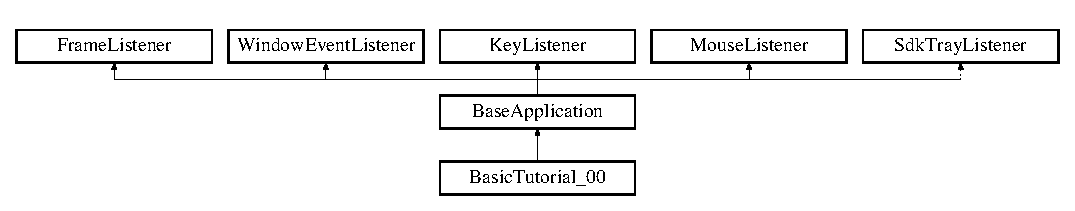
\includegraphics[height=2.382979cm]{class_basic_tutorial__00}
\end{center}
\end{figure}
\subsection*{Public Member Functions}
\begin{DoxyCompactItemize}
\item 
\hyperlink{class_basic_tutorial__00_a6b55068822076b28e7819b1878e95684}{Basic\+Tutorial\+\_\+00} (void)
\item 
virtual void \hyperlink{class_basic_tutorial__00_adc2454d9f8226e0958ecf702f355846e}{create\+Viewports} (void)
\item 
virtual void \hyperlink{class_basic_tutorial__00_a15a3d4673724ec99077ce992f996a550}{create\+Scene} (void)
\item 
virtual void \hyperlink{class_basic_tutorial__00_a1bf709417d654dffc2ea10987412b912}{create\+Camera} (void)
\item 
virtual void \hyperlink{class_basic_tutorial__00_aba97a29d983586d2dc8e108d3bccf721}{choose\+Scene\+Manager} (void)
\item 
virtual bool \hyperlink{class_basic_tutorial__00_a94e281a96584a25bf57b1c5e73737c81}{frame\+Started} (const Ogre\+::\+Frame\+Event \&evt)
\begin{DoxyCompactList}\small\item\em In the requirement of animation with key\+:0. \end{DoxyCompactList}\item 
virtual Vector3 \hyperlink{class_basic_tutorial__00_a90e8fc0b5789c3897a87b08e45bf6fe0}{move\+\_\+down} (Vector3, float)
\begin{DoxyCompactList}\small\item\em this function is for the key\+:0 animation \end{DoxyCompactList}\item 
virtual Vector3 \hyperlink{class_basic_tutorial__00_a3bec198c9f41ab006a1193311dfb4e0b}{move\+\_\+up} (Vector3, float)
\begin{DoxyCompactList}\small\item\em this function is for the key\+:0 animation \end{DoxyCompactList}\end{DoxyCompactItemize}
\subsection*{Protected Member Functions}
\begin{DoxyCompactItemize}
\item 
void \hyperlink{class_basic_tutorial__00_a6d4684502f2f7b2cf628a975d7750d8e}{create\+Viewport\+\_\+00} (void)
\begin{DoxyCompactList}\small\item\em Set the viewport with camera\mbox{[}0\mbox{]}. \end{DoxyCompactList}\item 
void \hyperlink{class_basic_tutorial__00_a2801a2f0d91d80b471da48344d2ccccf}{create\+Viewport\+\_\+01} (void)
\begin{DoxyCompactList}\small\item\em Set the viewport with camera\mbox{[}1\mbox{]}. \end{DoxyCompactList}\item 
void \hyperlink{class_basic_tutorial__00_a3479c50dbf8dc06a7ea77014eb94c6e7}{create\+Camera\+\_\+00} ()
\item 
void \hyperlink{class_basic_tutorial__00_a8745a127adeb69fa769f832fd41412c0}{create\+Camera\+\_\+01} ()
\item 
void \hyperlink{class_basic_tutorial__00_aa84173e509858146cbfb98274c1ef56e}{create\+Scene\+\_\+00} ()
\begin{DoxyCompactList}\small\item\em First specify the scene manager by assign. \end{DoxyCompactList}\item 
void \hyperlink{class_basic_tutorial__00_aad14e1ca565797c4b7dcff31bc0e1494}{create\+Scene\+\_\+01} ()
\begin{DoxyCompactList}\small\item\em In the second scene I\textquotesingle{}ve done the following things\+: \end{DoxyCompactList}\item 
bool \hyperlink{class_basic_tutorial__00_adc1a0b32d78b1980b3ee51a1b1e1e69b}{key\+Pressed} (const O\+I\+S\+::\+Key\+Event \&arg)
\begin{DoxyCompactList}\small\item\em Handle the key event. \end{DoxyCompactList}\item 
bool \hyperlink{class_basic_tutorial__00_aacca7a0a2a5a0e0d007b9c6c30b4941b}{key\+Released} (const O\+I\+S\+::\+Key\+Event \&arg)
\end{DoxyCompactItemize}
\subsection*{Protected Attributes}
\begin{DoxyCompactItemize}
\item 
Ogre\+::\+Viewport $\ast$ \hyperlink{class_basic_tutorial__00_a6676a92b50e9b43634d4c66488537b73}{m\+Viewport\+Arr} \mbox{[}8\mbox{]}
\item 
Ogre\+::\+Camera $\ast$ \hyperlink{class_basic_tutorial__00_af8d457d912286a98c0975c52d4faf910}{m\+Camera\+Arr} \mbox{[}8\mbox{]}
\item 
Ogre\+::\+Scene\+Manager $\ast$ \hyperlink{class_basic_tutorial__00_a603779b6087698c57b7989e16d8a9b93}{m\+Scene\+Mgr\+Arr} \mbox{[}8\mbox{]}
\item 
Ogre\+Bites\+::\+Sdk\+Camera\+Man $\ast$ \hyperlink{class_basic_tutorial__00_a700c07f924c71e9fa1885a46f599d934}{m\+Camera\+Man\+Arr} \mbox{[}8\mbox{]}
\end{DoxyCompactItemize}


\subsection{Detailed Description}
3D Game Programming ~\newline
My Name\+: Li-\/\+Che Chien ~\newline
My ID\+: 0316235 ~\newline
My Email\+: \href{mailto:richard@hotmail.com}{\tt richard@hotmail.\+com} 

\subsection{Constructor \& Destructor Documentation}
\mbox{\Hypertarget{class_basic_tutorial__00_a6b55068822076b28e7819b1878e95684}\label{class_basic_tutorial__00_a6b55068822076b28e7819b1878e95684}} 
\index{Basic\+Tutorial\+\_\+00@{Basic\+Tutorial\+\_\+00}!Basic\+Tutorial\+\_\+00@{Basic\+Tutorial\+\_\+00}}
\index{Basic\+Tutorial\+\_\+00@{Basic\+Tutorial\+\_\+00}!Basic\+Tutorial\+\_\+00@{Basic\+Tutorial\+\_\+00}}
\subsubsection{\texorpdfstring{Basic\+Tutorial\+\_\+00()}{BasicTutorial\_00()}}
{\footnotesize\ttfamily Basic\+Tutorial\+\_\+00\+::\+Basic\+Tutorial\+\_\+00 (\begin{DoxyParamCaption}\item[{void}]{ }\end{DoxyParamCaption})}


\begin{DoxyCode}
31 \{\}
\end{DoxyCode}


\subsection{Member Function Documentation}
\mbox{\Hypertarget{class_basic_tutorial__00_aba97a29d983586d2dc8e108d3bccf721}\label{class_basic_tutorial__00_aba97a29d983586d2dc8e108d3bccf721}} 
\index{Basic\+Tutorial\+\_\+00@{Basic\+Tutorial\+\_\+00}!choose\+Scene\+Manager@{choose\+Scene\+Manager}}
\index{choose\+Scene\+Manager@{choose\+Scene\+Manager}!Basic\+Tutorial\+\_\+00@{Basic\+Tutorial\+\_\+00}}
\subsubsection{\texorpdfstring{choose\+Scene\+Manager()}{chooseSceneManager()}}
{\footnotesize\ttfamily void Basic\+Tutorial\+\_\+00\+::choose\+Scene\+Manager (\begin{DoxyParamCaption}\item[{void}]{ }\end{DoxyParamCaption})\hspace{0.3cm}{\ttfamily [virtual]}}



Reimplemented from \hyperlink{class_base_application_ad5bc9655041e1849a4c13f444a3712bd}{Base\+Application}.


\begin{DoxyCode}
34 \{
35     \hyperlink{class_basic_tutorial__00_a603779b6087698c57b7989e16d8a9b93}{mSceneMgrArr}[0] = \hyperlink{class_base_application_add84ba707dc6c57e6283f214b1274110}{mRoot}
36         ->createSceneManager(ST\_GENERIC, \textcolor{stringliteral}{"primary"});
37     \hyperlink{class_basic_tutorial__00_a603779b6087698c57b7989e16d8a9b93}{mSceneMgrArr}[1] = \hyperlink{class_base_application_add84ba707dc6c57e6283f214b1274110}{mRoot}
38         ->createSceneManager(ST\_GENERIC, \textcolor{stringliteral}{"secondary"});
39 \}
\end{DoxyCode}
\mbox{\Hypertarget{class_basic_tutorial__00_a1bf709417d654dffc2ea10987412b912}\label{class_basic_tutorial__00_a1bf709417d654dffc2ea10987412b912}} 
\index{Basic\+Tutorial\+\_\+00@{Basic\+Tutorial\+\_\+00}!create\+Camera@{create\+Camera}}
\index{create\+Camera@{create\+Camera}!Basic\+Tutorial\+\_\+00@{Basic\+Tutorial\+\_\+00}}
\subsubsection{\texorpdfstring{create\+Camera()}{createCamera()}}
{\footnotesize\ttfamily void Basic\+Tutorial\+\_\+00\+::create\+Camera (\begin{DoxyParamCaption}\item[{void}]{ }\end{DoxyParamCaption})\hspace{0.3cm}{\ttfamily [virtual]}}



Reimplemented from \hyperlink{class_base_application_afa9d51527763cf9aee9cd4e1b1039d55}{Base\+Application}.


\begin{DoxyCode}
261                                         \{
262     \textcolor{comment}{//Do not modify}
263     \hyperlink{class_basic_tutorial__00_a3479c50dbf8dc06a7ea77014eb94c6e7}{createCamera\_00}();
264     \hyperlink{class_basic_tutorial__00_a8745a127adeb69fa769f832fd41412c0}{createCamera\_01}();
265     \hyperlink{class_base_application_a9ae38dea6316058549151fff66a91fcd}{mCameraMan} = \hyperlink{class_basic_tutorial__00_a700c07f924c71e9fa1885a46f599d934}{mCameraManArr}[0];
266     \textcolor{comment}{//mCameraMan = mCameraManArr[1];}
267 \}
\end{DoxyCode}
\mbox{\Hypertarget{class_basic_tutorial__00_a3479c50dbf8dc06a7ea77014eb94c6e7}\label{class_basic_tutorial__00_a3479c50dbf8dc06a7ea77014eb94c6e7}} 
\index{Basic\+Tutorial\+\_\+00@{Basic\+Tutorial\+\_\+00}!create\+Camera\+\_\+00@{create\+Camera\+\_\+00}}
\index{create\+Camera\+\_\+00@{create\+Camera\+\_\+00}!Basic\+Tutorial\+\_\+00@{Basic\+Tutorial\+\_\+00}}
\subsubsection{\texorpdfstring{create\+Camera\+\_\+00()}{createCamera\_00()}}
{\footnotesize\ttfamily void Basic\+Tutorial\+\_\+00\+::create\+Camera\+\_\+00 (\begin{DoxyParamCaption}\item[{void}]{ }\end{DoxyParamCaption})\hspace{0.3cm}{\ttfamily [protected]}}


\begin{DoxyCode}
42 \{
43     \hyperlink{class_base_application_a8a7684f4f9a57ed3089048ad1a913b2d}{mSceneMgr} = \hyperlink{class_basic_tutorial__00_a603779b6087698c57b7989e16d8a9b93}{mSceneMgrArr}[0];
44     \hyperlink{class_base_application_a3829c6b12afe911e97e6b4524b33a38b}{mCamera} = \hyperlink{class_basic_tutorial__00_af8d457d912286a98c0975c52d4faf910}{mCameraArr}[0] = \hyperlink{class_base_application_a8a7684f4f9a57ed3089048ad1a913b2d}{mSceneMgr}->createCamera(\textcolor{stringliteral}{"PlayerCam"});
45     \hyperlink{class_base_application_a3829c6b12afe911e97e6b4524b33a38b}{mCamera}->setPosition(Ogre::Vector3(120,300,600));
46     \hyperlink{class_base_application_a3829c6b12afe911e97e6b4524b33a38b}{mCamera}->lookAt(Ogre::Vector3(120,0,0));
47     \hyperlink{class_base_application_a3829c6b12afe911e97e6b4524b33a38b}{mCamera}->setNearClipDistance(5);
48     \hyperlink{class_basic_tutorial__00_a700c07f924c71e9fa1885a46f599d934}{mCameraManArr}[0] = \textcolor{keyword}{new} OgreBites::SdkCameraMan(\hyperlink{class_base_application_a3829c6b12afe911e97e6b4524b33a38b}{mCamera});   \textcolor{comment}{// create a default
       camera controller}
49 \}
\end{DoxyCode}
\mbox{\Hypertarget{class_basic_tutorial__00_a8745a127adeb69fa769f832fd41412c0}\label{class_basic_tutorial__00_a8745a127adeb69fa769f832fd41412c0}} 
\index{Basic\+Tutorial\+\_\+00@{Basic\+Tutorial\+\_\+00}!create\+Camera\+\_\+01@{create\+Camera\+\_\+01}}
\index{create\+Camera\+\_\+01@{create\+Camera\+\_\+01}!Basic\+Tutorial\+\_\+00@{Basic\+Tutorial\+\_\+00}}
\subsubsection{\texorpdfstring{create\+Camera\+\_\+01()}{createCamera\_01()}}
{\footnotesize\ttfamily void Basic\+Tutorial\+\_\+00\+::create\+Camera\+\_\+01 (\begin{DoxyParamCaption}\item[{void}]{ }\end{DoxyParamCaption})\hspace{0.3cm}{\ttfamily [protected]}}


\begin{DoxyCode}
52 \{
53     \textcolor{comment}{// add your own stuff}
54     \hyperlink{class_base_application_a8a7684f4f9a57ed3089048ad1a913b2d}{mSceneMgr} = \hyperlink{class_basic_tutorial__00_a603779b6087698c57b7989e16d8a9b93}{mSceneMgrArr}[1];
55     \hyperlink{class_base_application_a3829c6b12afe911e97e6b4524b33a38b}{mCamera} = \hyperlink{class_basic_tutorial__00_af8d457d912286a98c0975c52d4faf910}{mCameraArr}[1] = \hyperlink{class_base_application_a8a7684f4f9a57ed3089048ad1a913b2d}{mSceneMgr}->createCamera(\textcolor{stringliteral}{"SceneTwoCam"});
56     \hyperlink{class_base_application_a3829c6b12afe911e97e6b4524b33a38b}{mCamera}->setPosition(Ogre::Vector3(0, 350, 0.001));
57     \hyperlink{class_base_application_a3829c6b12afe911e97e6b4524b33a38b}{mCamera}->lookAt(Ogre::Vector3(0, 0, 0));
58     \hyperlink{class_base_application_a3829c6b12afe911e97e6b4524b33a38b}{mCamera}->setNearClipDistance(5);
59 \}
\end{DoxyCode}
\mbox{\Hypertarget{class_basic_tutorial__00_a15a3d4673724ec99077ce992f996a550}\label{class_basic_tutorial__00_a15a3d4673724ec99077ce992f996a550}} 
\index{Basic\+Tutorial\+\_\+00@{Basic\+Tutorial\+\_\+00}!create\+Scene@{create\+Scene}}
\index{create\+Scene@{create\+Scene}!Basic\+Tutorial\+\_\+00@{Basic\+Tutorial\+\_\+00}}
\subsubsection{\texorpdfstring{create\+Scene()}{createScene()}}
{\footnotesize\ttfamily void Basic\+Tutorial\+\_\+00\+::create\+Scene (\begin{DoxyParamCaption}\item[{void}]{ }\end{DoxyParamCaption})\hspace{0.3cm}{\ttfamily [virtual]}}



Implements \hyperlink{class_base_application_aa97beeb4059b17d0ec22eae33286ec2d}{Base\+Application}.


\begin{DoxyCode}
269                                          \{
270     \textcolor{comment}{//Do not modify}
271     \hyperlink{class_basic_tutorial__00_aa84173e509858146cbfb98274c1ef56e}{createScene\_00}();
272     \hyperlink{class_basic_tutorial__00_aad14e1ca565797c4b7dcff31bc0e1494}{createScene\_01}();
273     \textcolor{comment}{//mSceneMgr = mSceneMgrArr[0]; // active SceneManager}
274     \hyperlink{class_base_application_a8a7684f4f9a57ed3089048ad1a913b2d}{mSceneMgr} = \hyperlink{class_basic_tutorial__00_a603779b6087698c57b7989e16d8a9b93}{mSceneMgrArr}[1]; \textcolor{comment}{// active SceneManager}
275     \textcolor{comment}{//}
276     \hyperlink{class_base_application_a3829c6b12afe911e97e6b4524b33a38b}{mCamera} = \hyperlink{class_basic_tutorial__00_af8d457d912286a98c0975c52d4faf910}{mCameraArr}[0];
277     \textcolor{comment}{//mCamera = mCameraArr[1];}
278 \}
\end{DoxyCode}
\mbox{\Hypertarget{class_basic_tutorial__00_aa84173e509858146cbfb98274c1ef56e}\label{class_basic_tutorial__00_aa84173e509858146cbfb98274c1ef56e}} 
\index{Basic\+Tutorial\+\_\+00@{Basic\+Tutorial\+\_\+00}!create\+Scene\+\_\+00@{create\+Scene\+\_\+00}}
\index{create\+Scene\+\_\+00@{create\+Scene\+\_\+00}!Basic\+Tutorial\+\_\+00@{Basic\+Tutorial\+\_\+00}}
\subsubsection{\texorpdfstring{create\+Scene\+\_\+00()}{createScene\_00()}}
{\footnotesize\ttfamily void Basic\+Tutorial\+\_\+00\+::create\+Scene\+\_\+00 (\begin{DoxyParamCaption}\item[{void}]{ }\end{DoxyParamCaption})\hspace{0.3cm}{\ttfamily [protected]}}



First specify the scene manager by assign. 

I create the plane with given attributes

also set the ambient light and shadow with given number

Then I start to create two pengiuns and ground and cubes and wall
\begin{DoxyEnumerate}
\item Create objects entity .
\item Create scene node in scene manager meanwhile set its position or angle.
\item Attach entity to scene node.
\end{DoxyEnumerate}

for 72 cubes using a for loop with given values and set its meterial with chrome and Sphere\+Mapped\+Rusty\+Steel.

After all objects created, I set two point light with different position. 

References PI.


\begin{DoxyCode}
87 \{
88     \hyperlink{class_base_application_a8a7684f4f9a57ed3089048ad1a913b2d}{mSceneMgr} = \hyperlink{class_basic_tutorial__00_a603779b6087698c57b7989e16d8a9b93}{mSceneMgrArr}[0];
89     \textcolor{keywordtype}{int} numCubes = 72;
90     \textcolor{keywordtype}{int} L = 255;
91 
92     \textcolor{comment}{// add your own stuff}
93     Plane plane(Vector3::UNIT\_Y, 0);
94     Plane plane1(Vector3::UNIT\_Z,0);
95 
96     MeshManager::getSingleton().createPlane(
97         \textcolor{stringliteral}{"ground"},
98         ResourceGroupManager::DEFAULT\_RESOURCE\_GROUP\_NAME,
99         plane,
100         1500,1500, \textcolor{comment}{// width, height}
101         20,20, \textcolor{comment}{// x- and y-segments}
102         \textcolor{keyword}{true}, \textcolor{comment}{// normal}
103         1, \textcolor{comment}{// num texture sets}
104         5,5, \textcolor{comment}{// x- and y-tiles}
105         Vector3::UNIT\_Z \textcolor{comment}{// upward vector}
106     ); 
107 
108      MeshManager::getSingleton().createPlane(
109         \textcolor{stringliteral}{"wall"},
110         ResourceGroupManager::DEFAULT\_RESOURCE\_GROUP\_NAME,
111         plane1,
112         1500,1500,
113         20,20,
114         \textcolor{keyword}{true},
115         1,
116         5,5,
117         Vector3::UNIT\_Y
118     );
119 
120     \hyperlink{class_base_application_a8a7684f4f9a57ed3089048ad1a913b2d}{mSceneMgr}->setAmbientLight(ColourValue(0.5,0.5,0.5));
121     \hyperlink{class_base_application_a8a7684f4f9a57ed3089048ad1a913b2d}{mSceneMgr}->setShadowTechnique(SHADOWTYPE\_STENCIL\_ADDITIVE);
122     Entity* entPenguin1 = \hyperlink{class_base_application_a8a7684f4f9a57ed3089048ad1a913b2d}{mSceneMgr}->createEntity(\textcolor{stringliteral}{"Pengiun1"},\textcolor{stringliteral}{"penguin.mesh"});
123     Entity* entPenguin2 = \hyperlink{class_base_application_a8a7684f4f9a57ed3089048ad1a913b2d}{mSceneMgr}->createEntity(\textcolor{stringliteral}{"Pengiun2"},\textcolor{stringliteral}{"penguin.mesh"});
124     Entity* entPlane1 = \hyperlink{class_base_application_a8a7684f4f9a57ed3089048ad1a913b2d}{mSceneMgr}->createEntity(\textcolor{stringliteral}{"Ground"},\textcolor{stringliteral}{"ground"});
125     Entity* entPlane2 = \hyperlink{class_base_application_a8a7684f4f9a57ed3089048ad1a913b2d}{mSceneMgr}->createEntity(\textcolor{stringliteral}{"Wall"}, \textcolor{stringliteral}{"wall"});
126     entPlane2->setCastShadows(\textcolor{keyword}{false});
127     entPlane2->setMaterialName(\textcolor{stringliteral}{"Examples/Rockwall"});
128 
129     SceneNode *node0 = \hyperlink{class_base_application_a8a7684f4f9a57ed3089048ad1a913b2d}{mSceneMgr}
130         ->getRootSceneNode()
131         ->createChildSceneNode();
132 
133     SceneNode *node1 = \hyperlink{class_base_application_a8a7684f4f9a57ed3089048ad1a913b2d}{mSceneMgr}
134         ->getRootSceneNode()
135         ->createChildSceneNode(
136             \textcolor{stringliteral}{"PengiunNode"},
137             Vector3(0.0, 50.0, 0.0));
138 
139     SceneNode *node2 = \hyperlink{class_base_application_a8a7684f4f9a57ed3089048ad1a913b2d}{mSceneMgr}
140         ->getRootSceneNode()
141         ->createChildSceneNode(
142             Vector3(150.0, 20.0, 0.0));
143 
144      SceneNode *node3 = \hyperlink{class_base_application_a8a7684f4f9a57ed3089048ad1a913b2d}{mSceneMgr}
145         ->getRootSceneNode()
146         ->createChildSceneNode();
147 
148     node1 -> scale(2,3,2);
149     node2 -> yaw(Degree(-90));
150     node3 -> setPosition(0,0,-750);
151     node0 -> attachObject(entPlane1);
152     node3 -> attachObject(entPlane2);
153     node1 -> attachObject(entPenguin1);
154     node2 -> attachObject(entPenguin2);
155 
156     \textcolor{keywordflow}{for} (\textcolor{keywordtype}{int} i = 0; i < numCubes; ++i) \{
157         String name;
158         genNameUsingIndex(\textcolor{stringliteral}{"c"}, i, name);
159         Entity *ent = \hyperlink{class_base_application_a8a7684f4f9a57ed3089048ad1a913b2d}{mSceneMgr}->createEntity(name, \textcolor{stringliteral}{"cube.mesh"});
160         ent->setMaterialName(\textcolor{stringliteral}{"Examples/SphereMappedRustySteel"});
161         AxisAlignedBox bb = ent->getBoundingBox();
162         \textcolor{keywordtype}{float} cubeSize = bb.getMaximum().x - bb.getMinimum().x;
163         \textcolor{comment}{//x = 0, y = 0, z = -125;}
164         SceneNode *snode = \hyperlink{class_base_application_a8a7684f4f9a57ed3089048ad1a913b2d}{mSceneMgr}
165         ->getRootSceneNode()
166         ->createChildSceneNode();
167         snode->attachObject(ent);
168         \textcolor{keywordtype}{double} fx = i/(double) (numCubes-1); \textcolor{comment}{// in range [0,1]}
169         \textcolor{keywordtype}{double} h = (1+sin(fx*\hyperlink{_tutorial_application_8cpp_aa08a577393243b86dfd2a97e61443673}{PI}*4))*50; \textcolor{comment}{// height}
170         \textcolor{keywordtype}{double} circle\_radius = 100;
171         \textcolor{keywordtype}{double} x1 = circle\_radius*cos(fx*\hyperlink{_tutorial_application_8cpp_aa08a577393243b86dfd2a97e61443673}{PI}*2);
172         \textcolor{keywordtype}{double} z1 = circle\_radius*sin(fx*\hyperlink{_tutorial_application_8cpp_aa08a577393243b86dfd2a97e61443673}{PI}*2);
173         Real unitF = 1.0/cubeSize/numCubes*L*0.8;
174         snode->scale(unitF, h/cubeSize, unitF);
175         snode->setPosition(x1, 50, z1);
176     \} 
177 
178     \textcolor{keywordflow}{for} (\textcolor{keywordtype}{int} i = 0; i < numCubes; ++i) \{
179         String name;
180         genNameUsingIndex(\textcolor{stringliteral}{"cc"}, i, name);
181         Entity *ent = \hyperlink{class_base_application_a8a7684f4f9a57ed3089048ad1a913b2d}{mSceneMgr}->createEntity(name, \textcolor{stringliteral}{"cube.mesh"});
182         ent->setMaterialName(\textcolor{stringliteral}{"Examples/Chrome"});
183         AxisAlignedBox bb = ent->getBoundingBox();
184         \textcolor{keywordtype}{float} cubeSize = bb.getMaximum().x - bb.getMinimum().x;
185         \textcolor{comment}{//x = 0, y = 0, z = -125;}
186         SceneNode *snode = \hyperlink{class_base_application_a8a7684f4f9a57ed3089048ad1a913b2d}{mSceneMgr}
187         ->getRootSceneNode()
188         ->createChildSceneNode();
189         snode->attachObject(ent);
190         \textcolor{keywordtype}{double} fx = 2*i/(double) (numCubes-1); \textcolor{comment}{//i from 0 to numCubes-1}
191         \textcolor{keywordtype}{double} x = fx*L - L/2.0;
192         \textcolor{keywordtype}{double} h = (1+cos(fx*3.1415*2.0))*20; \textcolor{comment}{// height}
193         Real unitF = 1.0/cubeSize/numCubes*L*0.8;
194         snode->scale(unitF, h/cubeSize, unitF);
195         snode->setPosition(x, 20, 125);
196     \} 
197 
198     Light *light = \hyperlink{class_base_application_a8a7684f4f9a57ed3089048ad1a913b2d}{mSceneMgr} -> createLight(\textcolor{stringliteral}{"Light1"});
199     light->setType(Light::LT\_POINT);
200     light->setPosition(Vector3(150, 250, 100));
201     light->setDiffuseColour(0.0, 1.0, 0.0);
202     light->setSpecularColour(0.0, 1.0, 0.0);
203     Light *light2 = \hyperlink{class_base_application_a8a7684f4f9a57ed3089048ad1a913b2d}{mSceneMgr} -> createLight(\textcolor{stringliteral}{"Light2"});
204     light2->setType(Light::LT\_POINT);
205     light2->setPosition(Vector3(-150, 300, 250));
206     light2->setDiffuseColour(0.5, 0.5, 0.5);
207     light2->setSpecularColour(0.5, 0.5, 0.5);
208 
209 \}
\end{DoxyCode}
\mbox{\Hypertarget{class_basic_tutorial__00_aad14e1ca565797c4b7dcff31bc0e1494}\label{class_basic_tutorial__00_aad14e1ca565797c4b7dcff31bc0e1494}} 
\index{Basic\+Tutorial\+\_\+00@{Basic\+Tutorial\+\_\+00}!create\+Scene\+\_\+01@{create\+Scene\+\_\+01}}
\index{create\+Scene\+\_\+01@{create\+Scene\+\_\+01}!Basic\+Tutorial\+\_\+00@{Basic\+Tutorial\+\_\+00}}
\subsubsection{\texorpdfstring{create\+Scene\+\_\+01()}{createScene\_01()}}
{\footnotesize\ttfamily void Basic\+Tutorial\+\_\+00\+::create\+Scene\+\_\+01 (\begin{DoxyParamCaption}\item[{void}]{ }\end{DoxyParamCaption})\hspace{0.3cm}{\ttfamily [protected]}}



In the second scene I\textquotesingle{}ve done the following things\+: 


\begin{DoxyEnumerate}
\item Set Ambient light black(0,0,0) and shadow
\item Create point light
\item Create a plane and a cube entity with new material -\/ green
\item Scale the cube with (0.\+5,0.\+5,0.\+5) and attach to scene node 
\end{DoxyEnumerate}
\begin{DoxyCode}
212 \{
213     \textcolor{comment}{// add your own stuff}
214     \hyperlink{class_base_application_a8a7684f4f9a57ed3089048ad1a913b2d}{mSceneMgr} = \hyperlink{class_basic_tutorial__00_a603779b6087698c57b7989e16d8a9b93}{mSceneMgrArr}[1];
215     \hyperlink{class_base_application_a8a7684f4f9a57ed3089048ad1a913b2d}{mSceneMgr}->setAmbientLight(ColourValue(0,0,0));
216     \hyperlink{class_base_application_a8a7684f4f9a57ed3089048ad1a913b2d}{mSceneMgr}->setShadowTechnique(SHADOWTYPE\_STENCIL\_ADDITIVE);
217 
218     Light *light = \hyperlink{class_base_application_a8a7684f4f9a57ed3089048ad1a913b2d}{mSceneMgr} -> createLight(\textcolor{stringliteral}{"Light3"});
219     light->setType(Light::LT\_POINT);
220     light->setPosition(Vector3(100, 150, 250));
221     light->setDiffuseColour(0.0, 0.0, 1.0); \textcolor{comment}{//blue}
222     light->setSpecularColour(0.0,0.0, 1.0); \textcolor{comment}{//blue}
223 
224     Plane plane(Vector3::UNIT\_Y, 0);
225     MeshManager::getSingleton().createPlane(
226         \textcolor{stringliteral}{"plane"},
227         ResourceGroupManager::DEFAULT\_RESOURCE\_GROUP\_NAME,
228         plane,
229         1500,1500, \textcolor{comment}{// width, height}
230         20,20, \textcolor{comment}{// x- and y-segments}
231         \textcolor{keyword}{true}, \textcolor{comment}{// normal}
232         1, \textcolor{comment}{// num texture sets}
233         5,5, \textcolor{comment}{// x- and y-tiles}
234         Vector3::UNIT\_Z \textcolor{comment}{// upward vector}
235     ); 
236     Entity* entPlane = \hyperlink{class_base_application_a8a7684f4f9a57ed3089048ad1a913b2d}{mSceneMgr}->createEntity(\textcolor{stringliteral}{"Plane"},\textcolor{stringliteral}{"plane"});
237     Entity* ent = \hyperlink{class_base_application_a8a7684f4f9a57ed3089048ad1a913b2d}{mSceneMgr}->createEntity(\textcolor{stringliteral}{"Cube"},\textcolor{stringliteral}{"cube.mesh"});
238     ent->setMaterialName(\textcolor{stringliteral}{"Examples/green"});
239 
240     SceneNode *node = \hyperlink{class_base_application_a8a7684f4f9a57ed3089048ad1a913b2d}{mSceneMgr}
241         ->getRootSceneNode()
242         ->createChildSceneNode();
243 
244     SceneNode *node1 = \hyperlink{class_base_application_a8a7684f4f9a57ed3089048ad1a913b2d}{mSceneMgr}
245         ->getRootSceneNode()
246         ->createChildSceneNode(
247             Vector3(50.0, 0.0, 0.0));
248 
249     node1 -> scale(0.5,0.5,0.5);
250     node -> attachObject(entPlane);
251     node1 -> attachObject(ent);
252 \}
\end{DoxyCode}
\mbox{\Hypertarget{class_basic_tutorial__00_a6d4684502f2f7b2cf628a975d7750d8e}\label{class_basic_tutorial__00_a6d4684502f2f7b2cf628a975d7750d8e}} 
\index{Basic\+Tutorial\+\_\+00@{Basic\+Tutorial\+\_\+00}!create\+Viewport\+\_\+00@{create\+Viewport\+\_\+00}}
\index{create\+Viewport\+\_\+00@{create\+Viewport\+\_\+00}!Basic\+Tutorial\+\_\+00@{Basic\+Tutorial\+\_\+00}}
\subsubsection{\texorpdfstring{create\+Viewport\+\_\+00()}{createViewport\_00()}}
{\footnotesize\ttfamily void Basic\+Tutorial\+\_\+00\+::create\+Viewport\+\_\+00 (\begin{DoxyParamCaption}\item[{void}]{ }\end{DoxyParamCaption})\hspace{0.3cm}{\ttfamily [protected]}}



Set the viewport with camera\mbox{[}0\mbox{]}. 

Set the background blue(0,0,1) and Z-\/order with default 0 (at the bottom)

and add it to the viewport arr. 
\begin{DoxyCode}
63 \{
64     \hyperlink{class_base_application_a3829c6b12afe911e97e6b4524b33a38b}{mCamera} = \hyperlink{class_basic_tutorial__00_af8d457d912286a98c0975c52d4faf910}{mCameraArr}[0];
65     Ogre::Viewport* vp = \hyperlink{class_base_application_ac5d8e9c81e036897bc82f81eff8c570f}{mWindow}->addViewport(\hyperlink{class_base_application_a3829c6b12afe911e97e6b4524b33a38b}{mCamera});
66     vp->setBackgroundColour(Ogre::ColourValue(0,0.0,1.0));
67     \hyperlink{class_base_application_a3829c6b12afe911e97e6b4524b33a38b}{mCamera}->setAspectRatio(
68         Ogre::Real(vp->getActualWidth()) / Ogre::Real(vp->getActualHeight()));
69 
70     \hyperlink{class_basic_tutorial__00_a6676a92b50e9b43634d4c66488537b73}{mViewportArr}[0] = vp;
71 \}
\end{DoxyCode}
\mbox{\Hypertarget{class_basic_tutorial__00_a2801a2f0d91d80b471da48344d2ccccf}\label{class_basic_tutorial__00_a2801a2f0d91d80b471da48344d2ccccf}} 
\index{Basic\+Tutorial\+\_\+00@{Basic\+Tutorial\+\_\+00}!create\+Viewport\+\_\+01@{create\+Viewport\+\_\+01}}
\index{create\+Viewport\+\_\+01@{create\+Viewport\+\_\+01}!Basic\+Tutorial\+\_\+00@{Basic\+Tutorial\+\_\+00}}
\subsubsection{\texorpdfstring{create\+Viewport\+\_\+01()}{createViewport\_01()}}
{\footnotesize\ttfamily void Basic\+Tutorial\+\_\+00\+::create\+Viewport\+\_\+01 (\begin{DoxyParamCaption}\item[{void}]{ }\end{DoxyParamCaption})\hspace{0.3cm}{\ttfamily [protected]}}



Set the viewport with camera\mbox{[}1\mbox{]}. 

Set the background blue(0,0,1) and Z-\/order with 1 (at the top)

and add it to the viewport arr. 
\begin{DoxyCode}
74 \{
75     \textcolor{comment}{// add your own stuff}
76     \hyperlink{class_base_application_a3829c6b12afe911e97e6b4524b33a38b}{mCamera} = \hyperlink{class_basic_tutorial__00_af8d457d912286a98c0975c52d4faf910}{mCameraArr}[1];
77     Ogre::Viewport* vp = \hyperlink{class_base_application_ac5d8e9c81e036897bc82f81eff8c570f}{mWindow}->addViewport(\hyperlink{class_base_application_a3829c6b12afe911e97e6b4524b33a38b}{mCamera},1,0.75,0,0.25,0.25);
78     vp->setOverlaysEnabled(\textcolor{keyword}{false});
79     vp->setBackgroundColour(Ogre::ColourValue(0,0.0,1.0));
80     \hyperlink{class_base_application_a3829c6b12afe911e97e6b4524b33a38b}{mCamera}->setAspectRatio(
81         Ogre::Real(vp->getActualWidth()) / Ogre::Real(vp->getActualHeight()));
82 
83     \hyperlink{class_basic_tutorial__00_a6676a92b50e9b43634d4c66488537b73}{mViewportArr}[1] = vp;
84 \}
\end{DoxyCode}
\mbox{\Hypertarget{class_basic_tutorial__00_adc2454d9f8226e0958ecf702f355846e}\label{class_basic_tutorial__00_adc2454d9f8226e0958ecf702f355846e}} 
\index{Basic\+Tutorial\+\_\+00@{Basic\+Tutorial\+\_\+00}!create\+Viewports@{create\+Viewports}}
\index{create\+Viewports@{create\+Viewports}!Basic\+Tutorial\+\_\+00@{Basic\+Tutorial\+\_\+00}}
\subsubsection{\texorpdfstring{create\+Viewports()}{createViewports()}}
{\footnotesize\ttfamily void Basic\+Tutorial\+\_\+00\+::create\+Viewports (\begin{DoxyParamCaption}\item[{void}]{ }\end{DoxyParamCaption})\hspace{0.3cm}{\ttfamily [virtual]}}



Reimplemented from \hyperlink{class_base_application_a1f8f6730cae6ec769d8730b1af48486e}{Base\+Application}.


\begin{DoxyCode}
255 \{
256     \textcolor{comment}{//Do not modify}
257     \hyperlink{class_basic_tutorial__00_a6d4684502f2f7b2cf628a975d7750d8e}{createViewport\_00}();
258     \hyperlink{class_basic_tutorial__00_a2801a2f0d91d80b471da48344d2ccccf}{createViewport\_01}();
259 \}
\end{DoxyCode}
\mbox{\Hypertarget{class_basic_tutorial__00_a94e281a96584a25bf57b1c5e73737c81}\label{class_basic_tutorial__00_a94e281a96584a25bf57b1c5e73737c81}} 
\index{Basic\+Tutorial\+\_\+00@{Basic\+Tutorial\+\_\+00}!frame\+Started@{frame\+Started}}
\index{frame\+Started@{frame\+Started}!Basic\+Tutorial\+\_\+00@{Basic\+Tutorial\+\_\+00}}
\subsubsection{\texorpdfstring{frame\+Started()}{frameStarted()}}
{\footnotesize\ttfamily bool Basic\+Tutorial\+\_\+00\+::frame\+Started (\begin{DoxyParamCaption}\item[{const Ogre\+::\+Frame\+Event \&}]{evt }\end{DoxyParamCaption})\hspace{0.3cm}{\ttfamily [virtual]}}



In the requirement of animation with key\+:0. 

I use several flags to indicates the state

first I use zero\+\_\+flag to check whether key\+:0 being click so animation starts

then I use time\+\_\+step as a counter to count the stage during animation

every fram time\+\_\+step will increase by 0.\+002, which is the appropriate value I figured out from repeating tests

and then I use a pengiun\+State flag to indicate whether its moving up or down

if up, it couldnt exceed 280, if down, it couldnt be lower than 0. 

References pengiun\+State, time\+\_\+step, and zero\+\_\+flag.


\begin{DoxyCode}
451 \{
452     \textcolor{keywordtype}{bool} flg = Ogre::FrameListener::frameStarted(evt);
453     \textcolor{comment}{// add your own stuff}
454     \textcolor{keywordflow}{if} (\hyperlink{_tutorial_application_8cpp_a99a5608017531b46cd3234d001ec1dcb}{zero\_flag})\{
455         \hyperlink{class_base_application_a8a7684f4f9a57ed3089048ad1a913b2d}{mSceneMgr} = \hyperlink{class_basic_tutorial__00_a603779b6087698c57b7989e16d8a9b93}{mSceneMgrArr}[0];
456         Entity* pengiun = \hyperlink{class_base_application_a8a7684f4f9a57ed3089048ad1a913b2d}{mSceneMgr}->getEntity(\textcolor{stringliteral}{"Pengiun1"});
457         SceneNode *node1 = \hyperlink{class_base_application_a8a7684f4f9a57ed3089048ad1a913b2d}{mSceneMgr}
458             ->getSceneNode(\textcolor{stringliteral}{"PengiunNode"});
459 
460         Vector3 position = node1->getPosition();
461 
462         \textcolor{keywordflow}{if} (!\hyperlink{_tutorial_application_8cpp_a1bf2c695da5bfaa4bc465da5b204289c}{pengiunState})\{
463             position = \hyperlink{class_basic_tutorial__00_a90e8fc0b5789c3897a87b08e45bf6fe0}{move\_down}(position, \hyperlink{_tutorial_application_8cpp_a4feca29d7349adc765dcdf44d396d46a}{time\_step});
464             \textcolor{keywordflow}{if} (position.y < 0)\{
465                 \hyperlink{_tutorial_application_8cpp_a4feca29d7349adc765dcdf44d396d46a}{time\_step} = 0;
466                 \hyperlink{_tutorial_application_8cpp_a1bf2c695da5bfaa4bc465da5b204289c}{pengiunState} = 1;
467             \}
468         \}
469 
470         \textcolor{keywordflow}{else} \textcolor{keywordflow}{if} (\hyperlink{_tutorial_application_8cpp_a1bf2c695da5bfaa4bc465da5b204289c}{pengiunState})\{
471             position = \hyperlink{class_basic_tutorial__00_a3bec198c9f41ab006a1193311dfb4e0b}{move\_up}(position, \hyperlink{_tutorial_application_8cpp_a4feca29d7349adc765dcdf44d396d46a}{time\_step});
472             \textcolor{keywordflow}{if} (position.y > 280)\{
473                 \hyperlink{_tutorial_application_8cpp_a4feca29d7349adc765dcdf44d396d46a}{time\_step} = 0;
474                 \hyperlink{_tutorial_application_8cpp_a1bf2c695da5bfaa4bc465da5b204289c}{pengiunState} = 0;
475             \}
476         \}
477 
478         node1->setPosition(position);
479         \hyperlink{_tutorial_application_8cpp_a4feca29d7349adc765dcdf44d396d46a}{time\_step} += 0.002;
480     \}
481     \textcolor{keywordflow}{return} flg;
482 \}
\end{DoxyCode}
\mbox{\Hypertarget{class_basic_tutorial__00_adc1a0b32d78b1980b3ee51a1b1e1e69b}\label{class_basic_tutorial__00_adc1a0b32d78b1980b3ee51a1b1e1e69b}} 
\index{Basic\+Tutorial\+\_\+00@{Basic\+Tutorial\+\_\+00}!key\+Pressed@{key\+Pressed}}
\index{key\+Pressed@{key\+Pressed}!Basic\+Tutorial\+\_\+00@{Basic\+Tutorial\+\_\+00}}
\subsubsection{\texorpdfstring{key\+Pressed()}{keyPressed()}}
{\footnotesize\ttfamily bool Basic\+Tutorial\+\_\+00\+::key\+Pressed (\begin{DoxyParamCaption}\item[{const O\+I\+S\+::\+Key\+Event \&}]{arg }\end{DoxyParamCaption})\hspace{0.3cm}{\ttfamily [protected]}, {\ttfamily [virtual]}}



Handle the key event. 

From 1$\sim$5, just change the position and direction of camera

for M,N , I have to reset the viewport to new position and ratio, also change the z-\/order 

Reimplemented from \hyperlink{class_base_application_acfa977f04e435f18018ece805c1277ec}{Base\+Application}.



References Base\+Application\+::key\+Pressed(), and zero\+\_\+flag.


\begin{DoxyCode}
288 \{
289     \textcolor{keywordtype}{bool} flg = \textcolor{keyword}{true};
290     stringstream ss;
291     ss << arg.key;
292     String msg;
293     ss >> msg;
294     msg += \textcolor{stringliteral}{":*** keyPressed ***\(\backslash\)n"};
295     Ogre::LogManager::getSingletonPtr()->logMessage( msg );
296 
297     
298     \textcolor{keywordflow}{if} (arg.key == OIS::KC\_C ) \{
299         
300         ss.str(\textcolor{stringliteral}{""});
301         ss.clear();
302         
303         Vector3 pos = \hyperlink{class_base_application_a9ae38dea6316058549151fff66a91fcd}{mCameraMan}->getCamera()->getPosition(); 
304         ss << std::fixed << std::setprecision(2) 
305             << \textcolor{stringliteral}{"CameraPosition:"} 
306             << pos.x << \textcolor{stringliteral}{"\(\backslash\)t"} 
307             << pos.y << \textcolor{stringliteral}{"\(\backslash\)t"} 
308             << pos.z << \textcolor{stringliteral}{"\(\backslash\)n"};
309         Ogre::LogManager::getSingletonPtr()
310             ->logMessage( ss.str() );
311         \textcolor{comment}{//}
312         ss.str(\textcolor{stringliteral}{""});
313         ss.clear();
314         Vector3 dir = \hyperlink{class_base_application_a9ae38dea6316058549151fff66a91fcd}{mCameraMan}->getCamera()->getDirection();
315         ss << std::fixed << std::setprecision(2) 
316             << \textcolor{stringliteral}{"CameraDirection:"} 
317             << dir.x << \textcolor{stringliteral}{"\(\backslash\)t"} 
318             << dir.y << \textcolor{stringliteral}{"\(\backslash\)t"} 
319             << dir.z << \textcolor{stringliteral}{"\(\backslash\)n"};
320         Ogre::LogManager::getSingletonPtr()
321             ->logMessage( ss.str() );
322     \}
323 
324     \textcolor{keywordflow}{if} (arg.key == OIS::KC\_1 ) \{
325         \hyperlink{class_base_application_a9ae38dea6316058549151fff66a91fcd}{mCameraMan}->getCamera()
326             ->setPosition(Vector3(98.14,    450.69, 964.20));
327         \hyperlink{class_base_application_a9ae38dea6316058549151fff66a91fcd}{mCameraMan}->getCamera()
328             ->setDirection(Vector3(-0.01,   -0.30,  -0.95));
329     \}
330 
331     \textcolor{keywordflow}{if} (arg.key == OIS::KC\_2 ) \{
332         \textcolor{comment}{// add your own stuff}
333         \hyperlink{class_base_application_a9ae38dea6316058549151fff66a91fcd}{mCameraMan}->getCamera()
334             ->setPosition(Vector3(-1463.00, 606.45, -513.24));
335         \hyperlink{class_base_application_a9ae38dea6316058549151fff66a91fcd}{mCameraMan}->getCamera()
336             ->setDirection(Vector3(0.88, -0.47, 0.10));
337     \}
338 
339     \textcolor{keywordflow}{if} (arg.key == OIS::KC\_3 ) \{
340         \textcolor{comment}{// add your own stuff}
341         \hyperlink{class_base_application_a9ae38dea6316058549151fff66a91fcd}{mCameraMan}->getCamera()
342             ->setPosition(Vector3(-1356.16, 634.32, -964.51));
343         \hyperlink{class_base_application_a9ae38dea6316058549151fff66a91fcd}{mCameraMan}->getCamera()
344             ->setDirection(Vector3(0.71,    -0.44,  0.55));
345     \}
346 
347     \textcolor{keywordflow}{if} (arg.key == OIS::KC\_4 ) \{
348          \textcolor{comment}{// add your own stuff}
349         \hyperlink{class_base_application_a9ae38dea6316058549151fff66a91fcd}{mCameraMan}->getCamera()
350             ->setPosition(Vector3(40.39,    155.23, 251.20));
351         \hyperlink{class_base_application_a9ae38dea6316058549151fff66a91fcd}{mCameraMan}->getCamera()
352             ->setDirection(Vector3(-0.02,   -0.41,  -0.91));
353     \}
354 
355     \textcolor{keywordflow}{if} (arg.key == OIS::KC\_5 ) \{
356         \textcolor{comment}{// add your own stuff}
357         \hyperlink{class_base_application_a9ae38dea6316058549151fff66a91fcd}{mCameraMan}->getCamera()
358             ->setPosition(Vector3(19.94,    822.63, 30.79));
359         \hyperlink{class_base_application_a9ae38dea6316058549151fff66a91fcd}{mCameraMan}->getCamera()
360             ->setDirection(Vector3(0.00,    -0.99,  -0.11));
361     \}
362 
363     \textcolor{keywordflow}{if} (arg.key == OIS::KC\_M ) \{
364         
365        Camera *cam1 = \hyperlink{class_basic_tutorial__00_af8d457d912286a98c0975c52d4faf910}{mCameraArr}[0];
366        Camera *cam2 = \hyperlink{class_basic_tutorial__00_af8d457d912286a98c0975c52d4faf910}{mCameraArr}[1];
367 
368        \hyperlink{class_base_application_ac5d8e9c81e036897bc82f81eff8c570f}{mWindow}->removeViewport(\hyperlink{class_basic_tutorial__00_a6676a92b50e9b43634d4c66488537b73}{mViewportArr}[0]->getZOrder());
369        \hyperlink{class_base_application_ac5d8e9c81e036897bc82f81eff8c570f}{mWindow}->removeViewport(\hyperlink{class_basic_tutorial__00_a6676a92b50e9b43634d4c66488537b73}{mViewportArr}[1]->getZOrder());
370     Ogre::Viewport* vp = \hyperlink{class_base_application_ac5d8e9c81e036897bc82f81eff8c570f}{mWindow}->addViewport(cam2);
371     vp->setOverlaysEnabled(\textcolor{keyword}{false});
372     vp->setBackgroundColour(Ogre::ColourValue(0,0.0,1.0));
373     cam2->setAspectRatio(
374         Ogre::Real(vp->getActualWidth()) / Ogre::Real(vp->getActualHeight()));
375     \hyperlink{class_basic_tutorial__00_a6676a92b50e9b43634d4c66488537b73}{mViewportArr}[1] = vp;
376 
377     vp = \hyperlink{class_base_application_ac5d8e9c81e036897bc82f81eff8c570f}{mWindow}->addViewport(
378         cam1,
379         1,
380         0,
381         0,
382         0.5,
383         0.2);
384     vp->setBackgroundColour(Ogre::ColourValue(0,0.5,0.0));
385     cam1->setAspectRatio(
386         Ogre::Real(vp->getActualWidth()) / Ogre::Real(vp->getActualHeight()));
387         \hyperlink{class_basic_tutorial__00_a6676a92b50e9b43634d4c66488537b73}{mViewportArr}[0] = vp;          
388     \}
389 
390     \textcolor{keywordflow}{if} (arg.key == OIS::KC\_N ) \{
391         \textcolor{comment}{// add your own stuff}
392        Camera *cam1 = \hyperlink{class_basic_tutorial__00_af8d457d912286a98c0975c52d4faf910}{mCameraArr}[0];
393        Camera *cam2 = \hyperlink{class_basic_tutorial__00_af8d457d912286a98c0975c52d4faf910}{mCameraArr}[1];
394 
395        \hyperlink{class_base_application_ac5d8e9c81e036897bc82f81eff8c570f}{mWindow}->removeViewport(\hyperlink{class_basic_tutorial__00_a6676a92b50e9b43634d4c66488537b73}{mViewportArr}[0]->getZOrder());
396        \hyperlink{class_base_application_ac5d8e9c81e036897bc82f81eff8c570f}{mWindow}->removeViewport(\hyperlink{class_basic_tutorial__00_a6676a92b50e9b43634d4c66488537b73}{mViewportArr}[1]->getZOrder());
397     Ogre::Viewport* vp = \hyperlink{class_base_application_ac5d8e9c81e036897bc82f81eff8c570f}{mWindow}->addViewport(cam2,
398         1,
399         0.5,
400         0.3,
401         0.5,
402         0.2);
403     vp->setOverlaysEnabled(\textcolor{keyword}{false});
404     vp->setBackgroundColour(Ogre::ColourValue(0,0.0,1.0));
405     cam2->setAspectRatio(
406         Ogre::Real(vp->getActualWidth()) / Ogre::Real(vp->getActualHeight()));
407     \hyperlink{class_basic_tutorial__00_a6676a92b50e9b43634d4c66488537b73}{mViewportArr}[1] = vp;    
408 
409     vp = \hyperlink{class_base_application_ac5d8e9c81e036897bc82f81eff8c570f}{mWindow}->addViewport(cam1);
410     vp->setBackgroundColour(Ogre::ColourValue(1.0,0.0,0.0));
411     cam1->setAspectRatio(
412         Ogre::Real(vp->getActualWidth()) / Ogre::Real(vp->getActualHeight()));
413     \hyperlink{class_basic_tutorial__00_a6676a92b50e9b43634d4c66488537b73}{mViewportArr}[0] = vp;     
414     \}
415 
416     \textcolor{keywordflow}{if} (arg.key == OIS::KC\_0 ) \{
417         \textcolor{keywordflow}{switch}(\hyperlink{_tutorial_application_8cpp_a99a5608017531b46cd3234d001ec1dcb}{zero\_flag})\{
418             \textcolor{keywordflow}{case} \textcolor{keyword}{true}:
419                 \hyperlink{_tutorial_application_8cpp_a99a5608017531b46cd3234d001ec1dcb}{zero\_flag} = \textcolor{keyword}{false};
420                 \textcolor{keywordflow}{break};
421             \textcolor{keywordflow}{case} \textcolor{keyword}{false}:
422                 \hyperlink{_tutorial_application_8cpp_a99a5608017531b46cd3234d001ec1dcb}{zero\_flag} = \textcolor{keyword}{true};
423                 \textcolor{keywordflow}{break};
424         \}
425     \}
426 
427     \textcolor{comment}{// Do not delete this line}
428     \hyperlink{class_base_application_acfa977f04e435f18018ece805c1277ec}{BaseApplication::keyPressed}(arg);
429 
430     \textcolor{keywordflow}{return} flg;
431 \}
\end{DoxyCode}
\mbox{\Hypertarget{class_basic_tutorial__00_aacca7a0a2a5a0e0d007b9c6c30b4941b}\label{class_basic_tutorial__00_aacca7a0a2a5a0e0d007b9c6c30b4941b}} 
\index{Basic\+Tutorial\+\_\+00@{Basic\+Tutorial\+\_\+00}!key\+Released@{key\+Released}}
\index{key\+Released@{key\+Released}!Basic\+Tutorial\+\_\+00@{Basic\+Tutorial\+\_\+00}}
\subsubsection{\texorpdfstring{key\+Released()}{keyReleased()}}
{\footnotesize\ttfamily bool Basic\+Tutorial\+\_\+00\+::key\+Released (\begin{DoxyParamCaption}\item[{const O\+I\+S\+::\+Key\+Event \&}]{arg }\end{DoxyParamCaption})\hspace{0.3cm}{\ttfamily [protected]}, {\ttfamily [virtual]}}



Reimplemented from \hyperlink{class_base_application_aba5c7c9dea7a0efc58b89310bae547e5}{Base\+Application}.



References Base\+Application\+::key\+Released().


\begin{DoxyCode}
435 \{
436     \textcolor{keywordtype}{bool} flg = \textcolor{keyword}{true};
437     stringstream ss;
438     ss << arg.key;
439     String msg;
440     ss >> msg;
441     msg += \textcolor{stringliteral}{":*** keyReleased ***\(\backslash\)n"};
442     
443     Ogre::LogManager::getSingletonPtr()->logMessage( msg );
444 
445     \hyperlink{class_base_application_aba5c7c9dea7a0efc58b89310bae547e5}{BaseApplication::keyReleased}(arg);
446 
447     \textcolor{keywordflow}{return} flg;
448 \}
\end{DoxyCode}
\mbox{\Hypertarget{class_basic_tutorial__00_a90e8fc0b5789c3897a87b08e45bf6fe0}\label{class_basic_tutorial__00_a90e8fc0b5789c3897a87b08e45bf6fe0}} 
\index{Basic\+Tutorial\+\_\+00@{Basic\+Tutorial\+\_\+00}!move\+\_\+down@{move\+\_\+down}}
\index{move\+\_\+down@{move\+\_\+down}!Basic\+Tutorial\+\_\+00@{Basic\+Tutorial\+\_\+00}}
\subsubsection{\texorpdfstring{move\+\_\+down()}{move\_down()}}
{\footnotesize\ttfamily Vector3 Basic\+Tutorial\+\_\+00\+::move\+\_\+down (\begin{DoxyParamCaption}\item[{Vector3}]{pos,  }\item[{float}]{time\+\_\+step }\end{DoxyParamCaption})\hspace{0.3cm}{\ttfamily [virtual]}}



this function is for the key\+:0 animation 

which calculates the new position when pengiun move down. 

References time\+\_\+step.


\begin{DoxyCode}
484                                                                \{
485     Vector3 velocity = Vector3(0.0,0.0,0.0);
486     Vector3 acceleration = Vector3(0.0, -50.8, 0.0);
487     
488     velocity += acceleration*\hyperlink{_tutorial_application_8cpp_a4feca29d7349adc765dcdf44d396d46a}{time\_step};
489     \textcolor{keywordflow}{return} pos + velocity*\hyperlink{_tutorial_application_8cpp_a4feca29d7349adc765dcdf44d396d46a}{time\_step};
490 \}
\end{DoxyCode}
\mbox{\Hypertarget{class_basic_tutorial__00_a3bec198c9f41ab006a1193311dfb4e0b}\label{class_basic_tutorial__00_a3bec198c9f41ab006a1193311dfb4e0b}} 
\index{Basic\+Tutorial\+\_\+00@{Basic\+Tutorial\+\_\+00}!move\+\_\+up@{move\+\_\+up}}
\index{move\+\_\+up@{move\+\_\+up}!Basic\+Tutorial\+\_\+00@{Basic\+Tutorial\+\_\+00}}
\subsubsection{\texorpdfstring{move\+\_\+up()}{move\_up()}}
{\footnotesize\ttfamily Vector3 Basic\+Tutorial\+\_\+00\+::move\+\_\+up (\begin{DoxyParamCaption}\item[{Vector3}]{pos,  }\item[{float}]{time\+\_\+step }\end{DoxyParamCaption})\hspace{0.3cm}{\ttfamily [virtual]}}



this function is for the key\+:0 animation 

which calculates the new position when pengiun move up. 

References time\+\_\+step.


\begin{DoxyCode}
492                                                              \{
493     Vector3 velocity = Vector3(0,0,0);
494     Vector3 acceleration = Vector3(0.0, 20.8, 0.0);
495     
496     \textcolor{keywordflow}{if} (velocity.y <= 80)
497     velocity += acceleration*\hyperlink{_tutorial_application_8cpp_a4feca29d7349adc765dcdf44d396d46a}{time\_step};
498     \textcolor{keywordflow}{return} pos + velocity*\hyperlink{_tutorial_application_8cpp_a4feca29d7349adc765dcdf44d396d46a}{time\_step};
499 \}
\end{DoxyCode}


\subsection{Member Data Documentation}
\mbox{\Hypertarget{class_basic_tutorial__00_af8d457d912286a98c0975c52d4faf910}\label{class_basic_tutorial__00_af8d457d912286a98c0975c52d4faf910}} 
\index{Basic\+Tutorial\+\_\+00@{Basic\+Tutorial\+\_\+00}!m\+Camera\+Arr@{m\+Camera\+Arr}}
\index{m\+Camera\+Arr@{m\+Camera\+Arr}!Basic\+Tutorial\+\_\+00@{Basic\+Tutorial\+\_\+00}}
\subsubsection{\texorpdfstring{m\+Camera\+Arr}{mCameraArr}}
{\footnotesize\ttfamily Ogre\+::\+Camera$\ast$ Basic\+Tutorial\+\_\+00\+::m\+Camera\+Arr\mbox{[}8\mbox{]}\hspace{0.3cm}{\ttfamily [protected]}}

\mbox{\Hypertarget{class_basic_tutorial__00_a700c07f924c71e9fa1885a46f599d934}\label{class_basic_tutorial__00_a700c07f924c71e9fa1885a46f599d934}} 
\index{Basic\+Tutorial\+\_\+00@{Basic\+Tutorial\+\_\+00}!m\+Camera\+Man\+Arr@{m\+Camera\+Man\+Arr}}
\index{m\+Camera\+Man\+Arr@{m\+Camera\+Man\+Arr}!Basic\+Tutorial\+\_\+00@{Basic\+Tutorial\+\_\+00}}
\subsubsection{\texorpdfstring{m\+Camera\+Man\+Arr}{mCameraManArr}}
{\footnotesize\ttfamily Ogre\+Bites\+::\+Sdk\+Camera\+Man$\ast$ Basic\+Tutorial\+\_\+00\+::m\+Camera\+Man\+Arr\mbox{[}8\mbox{]}\hspace{0.3cm}{\ttfamily [protected]}}

\mbox{\Hypertarget{class_basic_tutorial__00_a603779b6087698c57b7989e16d8a9b93}\label{class_basic_tutorial__00_a603779b6087698c57b7989e16d8a9b93}} 
\index{Basic\+Tutorial\+\_\+00@{Basic\+Tutorial\+\_\+00}!m\+Scene\+Mgr\+Arr@{m\+Scene\+Mgr\+Arr}}
\index{m\+Scene\+Mgr\+Arr@{m\+Scene\+Mgr\+Arr}!Basic\+Tutorial\+\_\+00@{Basic\+Tutorial\+\_\+00}}
\subsubsection{\texorpdfstring{m\+Scene\+Mgr\+Arr}{mSceneMgrArr}}
{\footnotesize\ttfamily Ogre\+::\+Scene\+Manager$\ast$ Basic\+Tutorial\+\_\+00\+::m\+Scene\+Mgr\+Arr\mbox{[}8\mbox{]}\hspace{0.3cm}{\ttfamily [protected]}}

\mbox{\Hypertarget{class_basic_tutorial__00_a6676a92b50e9b43634d4c66488537b73}\label{class_basic_tutorial__00_a6676a92b50e9b43634d4c66488537b73}} 
\index{Basic\+Tutorial\+\_\+00@{Basic\+Tutorial\+\_\+00}!m\+Viewport\+Arr@{m\+Viewport\+Arr}}
\index{m\+Viewport\+Arr@{m\+Viewport\+Arr}!Basic\+Tutorial\+\_\+00@{Basic\+Tutorial\+\_\+00}}
\subsubsection{\texorpdfstring{m\+Viewport\+Arr}{mViewportArr}}
{\footnotesize\ttfamily Ogre\+::\+Viewport$\ast$ Basic\+Tutorial\+\_\+00\+::m\+Viewport\+Arr\mbox{[}8\mbox{]}\hspace{0.3cm}{\ttfamily [protected]}}



The documentation for this class was generated from the following files\+:\begin{DoxyCompactItemize}
\item 
\hyperlink{_tutorial_application_8h}{Tutorial\+Application.\+h}\item 
\hyperlink{_tutorial_application_8cpp}{Tutorial\+Application.\+cpp}\end{DoxyCompactItemize}

\chapter{File Documentation}
\hypertarget{_base_application_8cpp}{}\section{Base\+Application.\+cpp File Reference}
\label{_base_application_8cpp}\index{Base\+Application.\+cpp@{Base\+Application.\+cpp}}
{\ttfamily \#include \char`\"{}Base\+Application.\+h\char`\"{}}\newline

\hypertarget{_base_application_8h}{}\section{Base\+Application.\+h File Reference}
\label{_base_application_8h}\index{Base\+Application.\+h@{Base\+Application.\+h}}
{\ttfamily \#include $<$Ogre\+Camera.\+h$>$}\newline
{\ttfamily \#include $<$Ogre\+Entity.\+h$>$}\newline
{\ttfamily \#include $<$Ogre\+Log\+Manager.\+h$>$}\newline
{\ttfamily \#include $<$Ogre\+Root.\+h$>$}\newline
{\ttfamily \#include $<$Ogre\+Viewport.\+h$>$}\newline
{\ttfamily \#include $<$Ogre\+Scene\+Manager.\+h$>$}\newline
{\ttfamily \#include $<$Ogre\+Render\+Window.\+h$>$}\newline
{\ttfamily \#include $<$Ogre\+Config\+File.\+h$>$}\newline
{\ttfamily \#include $<$O\+I\+S\+Events.\+h$>$}\newline
{\ttfamily \#include $<$O\+I\+S\+Input\+Manager.\+h$>$}\newline
{\ttfamily \#include $<$O\+I\+S\+Keyboard.\+h$>$}\newline
{\ttfamily \#include $<$O\+I\+S\+Mouse.\+h$>$}\newline
{\ttfamily \#include $<$Sdk\+Trays.\+h$>$}\newline
{\ttfamily \#include $<$Sdk\+Camera\+Man.\+h$>$}\newline
\subsection*{Classes}
\begin{DoxyCompactItemize}
\item 
class \hyperlink{class_base_application}{Base\+Application}
\end{DoxyCompactItemize}

\hypertarget{_tutorial_application_8cpp}{}\section{Tutorial\+Application.\+cpp File Reference}
\label{_tutorial_application_8cpp}\index{Tutorial\+Application.\+cpp@{Tutorial\+Application.\+cpp}}
{\ttfamily \#include \char`\"{}Tutorial\+Application.\+h\char`\"{}}\newline
{\ttfamily \#include \char`\"{}Basic\+Tools.\+h\char`\"{}}\newline
{\ttfamily \#include $<$iostream$>$}\newline
{\ttfamily \#include $<$sstream$>$}\newline
{\ttfamily \#include $<$string$>$}\newline
{\ttfamily \#include $<$iomanip$>$}\newline
\subsection*{Functions}
\begin{DoxyCompactItemize}
\item 
int \hyperlink{_tutorial_application_8cpp_a0ddf1224851353fc92bfbff6f499fa97}{main} (int argc, char $\ast$argv\mbox{[}$\,$\mbox{]})
\end{DoxyCompactItemize}
\subsection*{Variables}
\begin{DoxyCompactItemize}
\item 
const float \hyperlink{_tutorial_application_8cpp_aa08a577393243b86dfd2a97e61443673}{PI} = 3.\+141592654
\item 
float \hyperlink{_tutorial_application_8cpp_a4feca29d7349adc765dcdf44d396d46a}{time\+\_\+step} = 0
\item 
int \hyperlink{_tutorial_application_8cpp_a1bf2c695da5bfaa4bc465da5b204289c}{pengiun\+State} = 0
\item 
bool \hyperlink{_tutorial_application_8cpp_a99a5608017531b46cd3234d001ec1dcb}{zero\+\_\+flag} = false
\end{DoxyCompactItemize}


\subsection{Function Documentation}
\mbox{\Hypertarget{_tutorial_application_8cpp_a0ddf1224851353fc92bfbff6f499fa97}\label{_tutorial_application_8cpp_a0ddf1224851353fc92bfbff6f499fa97}} 
\index{Tutorial\+Application.\+cpp@{Tutorial\+Application.\+cpp}!main@{main}}
\index{main@{main}!Tutorial\+Application.\+cpp@{Tutorial\+Application.\+cpp}}
\subsubsection{\texorpdfstring{main()}{main()}}
{\footnotesize\ttfamily int main (\begin{DoxyParamCaption}\item[{int}]{argc,  }\item[{char $\ast$}]{argv\mbox{[}$\,$\mbox{]} }\end{DoxyParamCaption})}



References Base\+Application\+::go().


\begin{DoxyCode}
501                                  \{
502     \hyperlink{class_basic_tutorial__00}{BasicTutorial\_00} app;
503     app.\hyperlink{class_base_application_a8a14a65a29118dd75173aa68678a05e1}{go}();  
504     \textcolor{keywordflow}{return} 0;
505 \}
\end{DoxyCode}


\subsection{Variable Documentation}
\mbox{\Hypertarget{_tutorial_application_8cpp_a1bf2c695da5bfaa4bc465da5b204289c}\label{_tutorial_application_8cpp_a1bf2c695da5bfaa4bc465da5b204289c}} 
\index{Tutorial\+Application.\+cpp@{Tutorial\+Application.\+cpp}!pengiun\+State@{pengiun\+State}}
\index{pengiun\+State@{pengiun\+State}!Tutorial\+Application.\+cpp@{Tutorial\+Application.\+cpp}}
\subsubsection{\texorpdfstring{pengiun\+State}{pengiunState}}
{\footnotesize\ttfamily int pengiun\+State = 0}



Referenced by Basic\+Tutorial\+\_\+00\+::frame\+Started().

\mbox{\Hypertarget{_tutorial_application_8cpp_aa08a577393243b86dfd2a97e61443673}\label{_tutorial_application_8cpp_aa08a577393243b86dfd2a97e61443673}} 
\index{Tutorial\+Application.\+cpp@{Tutorial\+Application.\+cpp}!PI@{PI}}
\index{PI@{PI}!Tutorial\+Application.\+cpp@{Tutorial\+Application.\+cpp}}
\subsubsection{\texorpdfstring{PI}{PI}}
{\footnotesize\ttfamily const float PI = 3.\+141592654}



Referenced by Basic\+Tutorial\+\_\+00\+::create\+Scene\+\_\+00().

\mbox{\Hypertarget{_tutorial_application_8cpp_a4feca29d7349adc765dcdf44d396d46a}\label{_tutorial_application_8cpp_a4feca29d7349adc765dcdf44d396d46a}} 
\index{Tutorial\+Application.\+cpp@{Tutorial\+Application.\+cpp}!time\+\_\+step@{time\+\_\+step}}
\index{time\+\_\+step@{time\+\_\+step}!Tutorial\+Application.\+cpp@{Tutorial\+Application.\+cpp}}
\subsubsection{\texorpdfstring{time\+\_\+step}{time\_step}}
{\footnotesize\ttfamily float time\+\_\+step = 0}



Referenced by Basic\+Tutorial\+\_\+00\+::frame\+Started(), Basic\+Tutorial\+\_\+00\+::move\+\_\+down(), and Basic\+Tutorial\+\_\+00\+::move\+\_\+up().

\mbox{\Hypertarget{_tutorial_application_8cpp_a99a5608017531b46cd3234d001ec1dcb}\label{_tutorial_application_8cpp_a99a5608017531b46cd3234d001ec1dcb}} 
\index{Tutorial\+Application.\+cpp@{Tutorial\+Application.\+cpp}!zero\+\_\+flag@{zero\+\_\+flag}}
\index{zero\+\_\+flag@{zero\+\_\+flag}!Tutorial\+Application.\+cpp@{Tutorial\+Application.\+cpp}}
\subsubsection{\texorpdfstring{zero\+\_\+flag}{zero\_flag}}
{\footnotesize\ttfamily bool zero\+\_\+flag = false}



Referenced by Basic\+Tutorial\+\_\+00\+::frame\+Started(), and Basic\+Tutorial\+\_\+00\+::key\+Pressed().


\hypertarget{_tutorial_application_8h}{}\section{Tutorial\+Application.\+h File Reference}
\label{_tutorial_application_8h}\index{Tutorial\+Application.\+h@{Tutorial\+Application.\+h}}
{\ttfamily \#include \char`\"{}Base\+Application.\+h\char`\"{}}\newline
\subsection*{Classes}
\begin{DoxyCompactItemize}
\item 
class \hyperlink{class_basic_tutorial__00}{Basic\+Tutorial\+\_\+00}
\begin{DoxyCompactList}\small\item\em 3D Game Programming ~\newline
My Name\+: Li-\/\+Che Chien ~\newline
My ID\+: 0316235 ~\newline
My Email\+: \href{mailto:richard@hotmail.com}{\tt richard@hotmail.\+com} \end{DoxyCompactList}\end{DoxyCompactItemize}

%--- End generated contents ---

% Index
\backmatter
\newpage
\phantomsection
\clearemptydoublepage
\addcontentsline{toc}{chapter}{Index}
\printindex

\end{document}
